\documentclass[
	11pt, % Set the default font size, options include: 8pt, 9pt, 10pt, 11pt, 12pt, 14pt, 17pt, 20pt
	%t, % Uncomment to vertically align all slide content to the top of the slide, rather than the default centered
	%aspectratio=169, % Uncomment to set the aspect ratio to a 16:9 ratio which matches the aspect ratio of 1080p and 4K screens and projectors
]{beamer}
\usepackage{xcolor}
\graphicspath{{Images/}{./}} % Specifies where to look for included images (trailing slash required)
\usepackage{graphics,epstopdf}
\usepackage{graphicx}
\usepackage[final]{pdfpages}
%\addmediapath{/Users/hoangleson/Documents/Lecture in University /DHQG/DHQG-DuocLieu/Movies}
\usepackage[utf8]{vietnam}
%\usepackage[librsvg]{chemobabel}
\usepackage{sidecap}
\usepackage{chemfig}
\usepackage{ragged2e}
\usepackage{booktabs}
\usepackage{multirow}
\usepackage{booktabs}
\usepackage{setspace}
\usepackage{fancybox}
\usepackage{multimedia}
\usepackage[caption=false]{subfig}
\usepackage{blindtext}
\usepackage{varsfromjobname}
% Beamer comes with a number of default layout themes which change the colors and layouts of slides. Below is a list of all themes available, uncomment each in turn to see what they look like.

%\usetheme{default}
%\usetheme{AnnArbor}
%\usetheme{Antibes}
%\usetheme{Bergen}
%\usetheme{Berkeley}
%\usetheme{Berlin}
%\usetheme{Boadilla}
%\usetheme{CambridgeUS}
%\usetheme{Copenhagen}
%\usetheme{Darmstadt}
%\usetheme{Dresden}
%\usetheme{Frankfurt}
%\usetheme{Goettingen}
%\usetheme{Hannover}
%\usetheme{Ilmenau}
%\usetheme{JuanLesPins}
%\usetheme{Luebeck}
\usetheme{Madrid}
%\usetheme{Malmoe}
%\usetheme{Marburg}
%\usetheme{Montpellier}
%\usetheme{PaloAlto}
%\usetheme{Pittsburgh}
%\usetheme{Rochester}
%\usetheme{Singapore}
%\usetheme{Szeged}
%\usetheme{Warsaw}
%----------------------------------------------------------------------------------------
%	SELECT COLOR THEME
%----------------------------------------------------------------------------------------

% Beamer comes with a number of color themes that can be applied to any layout theme to change its colors. Uncomment each of these in turn to see how they change the colors of your selected layout theme.

%\usecolortheme{albatross}
%\usecolortheme{beaver}
%\usecolortheme{beetle}
%\usecolortheme{crane}
%\usecolortheme{dolphin}
%\usecolortheme{dove}
%\usecolortheme{fly}
%\usecolortheme{lily}
%\usecolortheme{monarca}
%\usecolortheme{seagull}
%\usecolortheme{seahorse}
%\usecolortheme{spruce}
%\usecolortheme{whale}
%\usecolortheme{wolverine}
%----------------------------------------------------------------------------------------
%	SELECT FONT THEME & FONTS
%----------------------------------------------------------------------------------------

% Beamer comes with several font themes to easily change the fonts used in various parts of the presentation. Review the comments beside each one to decide if you would like to use it. Note that additional options can be specified for several of these font themes, consult the beamer documentation for more information.

%\usefonttheme{default} % Typeset using the default sans serif font
%\usefonttheme{serif} % Typeset using the default serif font (make sure a sans font isn't being set as the default font if you use this option!)
\usefonttheme{structurebold} % Typeset important structure text (titles, headlines, footlines, sidebar, etc) in bold
%\usefonttheme{structureitalicserif} % Typeset important structure text (titles, headlines, footlines, sidebar, etc) in italic serif
%\usefonttheme{structuresmallcapsserif} % Typeset important structure text (titles, headlines, footlines, sidebar, etc) in small caps serif

%------------------------------------------------

%\usepackage{mathptmx} % Use the Times font for serif text
\usepackage{palatino} % Use the Palatino font for serif text

%\usepackage{helvet} % Use the Helvetica font for sans serif text
%\usepackage[default]{opensans} % Use the Open Sans font for sans serif text
%\usepackage[default]{FiraSans} % Use the Fira Sans font for sans serif text
%\usepackage[default]{lato} % Use the Lato font for sans serif text

%----------------------------------------------------------------------------------------
%	SELECT INNER THEME
%----------------------------------------------------------------------------------------

% Inner themes change the styling of internal slide elements, for example: bullet points, blocks, bibliography entries, title pages, theorems, etc. Uncomment each theme in turn to see what changes it makes to your presentation.

%\useinnertheme{default}
%\useinnertheme{circles}
%\useinnertheme{rectangles}
\useinnertheme{rounded}
%\useinnertheme{inmargin}

%----------------------------------------------------------------------------------------
%	SELECT OUTER THEME
%----------------------------------------------------------------------------------------

% Outer themes change the overall layout of slides, such as: header and footer lines, sidebars and slide titles. Uncomment each theme in turn to see what changes it makes to your presentation.

\useoutertheme{default}
%\useoutertheme{infolines}
%\useoutertheme{miniframes}
%\useoutertheme{smoothbars}
%\useoutertheme{sidebar}
%\useoutertheme{split}
%\useoutertheme{shadow}
%\useoutertheme{tree}
%\useoutertheme{smoothtree}

%\setbeamertemplate{footline} % Uncomment this line to remove the footer line in all slides
\setbeamertemplate{footline}[page number] % Uncomment this line to replace the footer line in all slides with a simple slide count
\setbeamertemplate{caption}{\raggedright\insertcaption\par}
\setbeamertemplate{navigation symbols}{} % Uncomment this line to remove the navigation symbols from the bottom of all slides
\addtobeamertemplate{block begin}{}{\justifying} 
%----------------------------------------------------------------------------------------
%	PRESENTATION INFORMATION
%----------------------------------------------------------------------------------------

\title[Dược cổ truyền]{DƯỢC CỔ TRUYỀN \newline Traditional Herbal Medicine} % The short title in the optional parameter appears at the bottom of every slide, the full title in the main parameter is only on the title page

%\subtitle{Dược liệu và các hợp chất từ tự nhiên} % Presentation subtitle, remove this command if a subtitle isn't required

\author[PhD. Hoàng Lê Sơn]{} % Presenter name(s), the optional parameter can contain a shortened version to appear on the bottom of every slide, while the main parameter will appear on the title slide

\institute[UC]{Bộ môn Dược liệu \& Dược cổ truyền\\ \smallskip \textit{sonhoang.ump@vnu.edu.vn}} % Your institution, the optional parameter can be used for the institution shorthand and will appear on the bottom of every slide after author names, while the required parameter is used on the title slide and can include your email address or additional information on separate lines
\usepackage{tikz}
\usetikzlibrary{trees}
%\titlegraphic { 
%\begin{tikzpicture}[overlay,remember picture]
%\node [xshift=0cm,yshift=4cm] at (current page.center){
%    
\includegraphics[width=1.2cm]{Logo.jpg}
%};
%\end{tikzpicture}
%}

% ------------- Creating a new block template ----------
\makeatletter
\def\th@newblock{%
  \normalfont 
  \def\inserttheoremblockenv{exampleblock}}
\theoremstyle{newblock}
\newtheorem{exercise}[theorem]{Ví dụ}
\makeatother


\date[\today]{\tiny\today} % Presentation date or conference/meeting name, the optional parameter can contain a shortened version to appear on the bottom of every slide, while the required parameter value is output to the title slide

%----------------------------------------------------------------------------------------
\setbeamercovered{transparent}
\usepackage{tikz}
\usetikzlibrary{overlay-beamer-styles}
 \tikzset{
    highlight on/.style={alt={#1{fill=red!80!black,color=red!80!black}{fill=gray!30!white,color=gray!30!white}}},
}
\usepackage{chronology}
\usepackage{blindtext}
%\setbeamertemplate{navigation symbols}{}

\begin{document}

\AtBeginSection[]{
  \begin{frame}
  \vfill
  \centering
  \begin{beamercolorbox}[sep=8pt,center,shadow=true,rounded=true]{title}
    \usebeamerfont{title}\insertsectionhead\par%
  \end{beamercolorbox}
  \vfill
  \end{frame}
}

%-------------------------------------------------------------------------------
%	TITLE SLIDE
%-------------------------------------------------------------------------------

\begin{frame}[plain]
	\titlepage % Output the title slide, automatically created using the text entered in the PRESENTATION INFORMATION block above
\end{frame}
\begin{frame}[plain]
	\frametitle{Phần A: Lý luận trong y học cổ truyền }
	\tableofcontents
\end{frame}



\begin{frame}{Tài liệu tham khảo}
	\begin{enumerate}
		\item Giáo trình Dược học cổ truyền, Trường Đại học Dược Hà nội.
		\item Dược điển Việt nam V, Bộ y tế.
		\item Chinese Herbal Medicines: Comparisons and Characteristics
		\item Chinese Herbal Formulas: Treatment Principles and Composition Strategies
		\item Chinese Traditional Herbal Medicine
		\item Combining Western Herbs and Chinese Medicine: Principles, Practice and Materia Medica
		\item The foundations of Chinese Medicine: A comprehensive text
	\end{enumerate}
\end{frame}
\begin{frame}{Tiểu luận theo nhóm}{}
	{\bf Mục tiêu:} Quan điểm đông y về một bệnh bất kỳ, cách trị bệnh và các thuốc\\
	{\bf Các nội dung cần có}
	\begin{itemize}
		\item Định nghĩa bệnh theo Bộ Y tế Việt Nam 
		\item Dịch nghĩa bệnh theo Đông Y: Chinese Herbal Formulas: Treatment Principles and Composition Strategies
		\item Giải thích các thuật ngữ xuất hiện: The foundations of Chinese Medicine: A comprehensive text
		\item Các dược liệu chữa bệnh này: Chinese Herbal Formulas: Treatment Principles and Composition Strategies
	\end{itemize}
\end{frame}
\begin{frame}{Tiểu luận cá nhân}{}
	{\bf Mục tiêu:} Cung cấp thông tin về cách sử dụng một vị thuốc giữa phương Tây, Trung Hoa và Việt nam\\
	{\bf Các nội dung cần có}
	\begin{itemize}
		\item Trong Dược điển Việt Nam V
		\item Combining Western Herbs and Chinese Medicine: Principles, Practice and Materia Medica
		\item Chinese Herbal Formulas: Treatment Principles and Composition Strategies
	\end{itemize}
\end{frame}	

%\AtBeginSection[]
%{
%    \begin{frame}
%        \frametitle{Đại cương về thuốc y học cổ truyền- Phân loại thuốc cổ truyền và Chế biến thuốc theo phương pháp cổ truyền}
%        \tableofcontents
%    \end{frame}
%}
\section{Vật chất cơ bản theo y học cổ truyền\newline The vital substances}
\begin{frame}[plain]
	\begin{columns}[T]
		\column{0.7\textwidth}
		\Huge{QI, BLOOD, FLUID}\\
		\huge{ESSENCE AND SHEN}\\
		\Large{Tinh-Khí-Thần-Huyết-Tân dịch}\\
		\column{0.3\textwidth}
			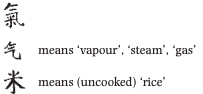
\includegraphics[width=\textwidth]{Images/Qi.png}	
	\end{columns}

	
	{\it Qi được dịch trong tiếng anh là "vital energy", "vital force", "material energy", hoặc "energy"}\\
	The ancient Chinese view of the body-mind.\\
	\begin{itemize}
		\item The concept of Qi in Chinese philosophy
		\item The concept of Qi in Chinese medicine
	\end{itemize}

\end{frame}

\begin{frame}[plain]
	\begin{columns}[T]
		\column{0.5\textwidth}
		\begin{itemize}
			\item Essence
			\begin{itemize}
				\item Pre-Heaven Essence
				\item Post-Heaven Essence
				\item The Kidney-Essence
			\end{itemize}
			\item Qi
			\begin{itemize}
				\item Original Qi (Yuan Qi)
				\item Food-Qi (Gu Qi)
				\item Gathering Qi (Zong Qi)
				\item True Qi (Zhen Qi)
				\item Central Qi (Zhong Qi)
				\item Upright Qi (Zheng Qi)
				\item Functions of Qi
				\item Direction of Qi movement
				\item Pathology of Qi
			\end{itemize}
		\end{itemize}
		\column{0.5\textwidth}
		\begin{itemize}
			\item Blood
			\begin{itemize}
				\item Source of Blood
				\item Functions of Blood
				\item Relation of Blood with internal organs
				\item Blood Qi relationship
				\item Blood Essence relationship
				\item Blood pathology
			\end{itemize}
			\item Body Fluids
			\begin{itemize}
				\item Source
				\item Relations with internal organs
				\item Types of Body Fluids
				\item Relation between Qi and Body Fluids
				\item Relation between Blood and Body Fluids
				\item Pathology of body fluids
			\end{itemize}
			\item Mind (Shen)
		\end{itemize}
	\end{columns}
\end{frame}
\begin{frame}{The concept of Qi in Chinese philosophy}{Qi trong triết học Trung Hoa}
	\begin{columns}[T]
		\column{0.5\textwidth}
		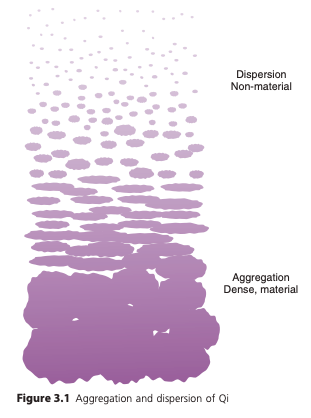
\includegraphics[width=\textwidth]{Images/Qi A and D.png}
		\column{0.5\textwidth}
		\only<1>{
		Triết học phương Tây luôn đề cập tới tính nhị nguyên như vật chất ý thức, linh hồn và thể xác.\\
		Qi được coi là hiện tượng cơ bản của thế giới, cung cấp tính chất liên tục giữa vật chất và ý thức.\\}
		{\footnotesize
		\only<2>{ Xun Kuang (c.313-238 bc) said: {\it Water and Fire have Qi but not life; plants and trees have life, but not knowledge; birds and animals have knowledge, but no sense of what are rights.}}
		\only<3>{ Lie Zi, a Daoist text from around 300 bc, said: {\it The 
		purer and lighter [elements], tending upwards, made the 
			heaven; the grosser and heavier [elements], tending downwards, made the earth}}
		\only<4>{ Huai Nan Zi (c.122 bc), another Daoist text,says:{\it Dao 
			originated from Emptiness and Emptiness produced the 
			universe. The universe produced Qi. That which was clear 
			and light drifted up to become heaven, and that which was 
			heavy and turbid solidified to form earth.}}
			\only<5>{ Wang Chong (ad 27-97): {\it Qi produces the human body just as water becomes ice. As water freezes into ice, so Qi coagulates to form the human body. When ice melts, it becomes water. When a person dies, he or she becomes spirit [shen] again. It is called spirit, just as melted ice changes its name to water.When it came to separation and differentiation, the pure 
			[elements] formed heaven, and the turbid ones formed 
			earth.}}
			\only<6>{Zhang Zai (ad 1020-1077) {\it Every birth is a condensation, 
			every death a dispersal. Birth is not a gain, death not a loss 
			… when condensed, Qi becomes a living being, when dispersed, it is the substratum of mutations}}
		\only<7>{Wang Fu Zhi (1619-1692): {\it Life is not 
		creation from nothing, and death is not complete dispersion 
		and destruction. [Despite the condensation and 
		dispersion of Qi] its original substance can neither be added 
		nor be lessened. All that is void and 
		empty is full of Qi which, in its state of condensation and 
		thus visible, is called being, but in its state of dispersion and 
		thus no longer visible, is called non-being. When dispersing Qi makes the Great Void, only regaining its original 
		misty feature but not perishing; when condensing, it 
		becomes the origin of all beings.}}}
	\end{columns}
\end{frame}

\begin{frame}{Qi trong y dược cổ truyền}{Qi is the 
	root of a human being}
	\begin{block}{}
		\begin{itemize}
			\item Qi is in a constant state of flux and in varying states of 
			aggregation. When condensed, Qi gives rise to physical 
			shape; when dispersed, Qi gives rise to subtle forms of 
			energy.
			\item  Qi is an energy which manifests simultaneously on the 
			physical and emotional-mental-spiritual level.
		\end{itemize}
	\end{block}
	\begin{columns}[T]
		\column{0.5\textwidth}
		\begin{center}
			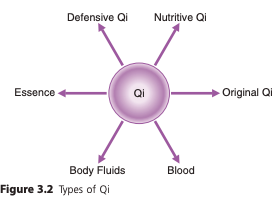
\includegraphics[height=0.5\textheight]{Images/Types of Qi.png}
		\end{center}
		\column{0.5\textwidth}
		{\bf Hai ý nghĩa của Qi trong cơ thể}
		\begin{itemize}
			\item The refined energy produced by the Internal Organs, 
			assuming different forms in different places.
			\item The functional activity of an Internal Organ (e.g. Liver-Qi, 
			Lung-Qi)
		\end{itemize}
	\end{columns}

\end{frame}


\begin{frame}{Tinh-Khí-Thần ESSENCE - QI- SHEN}{ Tam bảo đại diện cho ba trang thại ngưng tụ hoặc tổng hợp của khí, Tinh (SHEN) dày đặc nhất, khí (QI) tinh khiết hơn và thần (SHEN) tinh tế và phi vật chất nhất.}
	\begin{columns}[t]
		\begin{column}{0.7\textwidth}
			\begin{itemize}
				\item Các vật chất cần thiết cho sự sống giúp tạng, phủ, kinh lạc hoạt động.
				\item Tam bảo gồm Tinh, Khí, Thần là 3 vật chất cơ bản của sinh mệnh con người không thể tách rời, phân chia. Cùng tồn tại và cùng diệt vong
				\item Tinh là gốc của thần, có tinh mới có thần
				\item Tinh là mẹ của khí.
				\item Không có khí người không sống được
			\end{itemize}
		\end{column}
		\begin{column}{0.3\textwidth}
			\begin{center}
				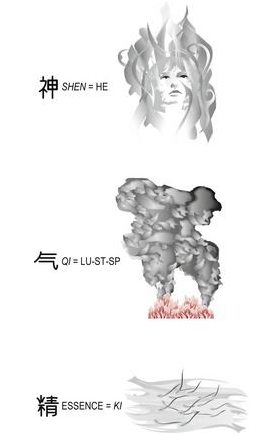
\includegraphics[width=\textwidth]{Images/The Three Treasures.png}
			\end{center}
		\end{column}
	\end{columns}
	\small{Zhang Jie Bin says: If the Essence is strong, Qi flourishes; if Qi flourishes, the Mind is whole. }
\end{frame}

\begin{frame}{Tinh-ESSENCE}
\begin{block}{Chức năng}
	Vật chất khởi nguồn của sinh mệnh và các hoạt động của cơ thể; là cơ
sở vật chất của nguyên khí con người chân âm và nguyên âm
\end{block}
\begin{columns}[T]
	\column{0.5\textwidth}
	\begin{itemize}
		\item Tinh tiên thiên: Bố mẹ sinh ra đã có tàng ở thận 
		\item Tinh hậu thiên: từ thực phẩm nuôi dưỡng cơ thể nuôi dưỡng tinh tiên thiên và lục phủ ngũ tạng, bì mao gân cốt. Dư thừa trữ tại thận 
		\item Tinh thận: Tinh tiên thiên và tinh hậu thiên giúp sinh trường phát triển, phát dục, di truyền
	\end{itemize}
	\column{0.5\textwidth}
	\begin{center}
		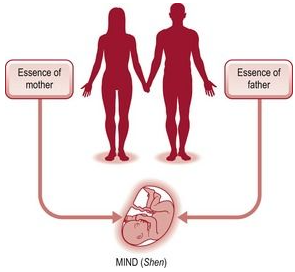
\includegraphics[width=\textwidth]{Images/Union of Essence to form mind.png}
	\end{center}
	Zhang Jie Bin says: {\it The two Essences, one Yin, one Yang, unite to form life; the Essences of mother and father unite to form the Mind.}
\end{columns}
\end{frame}

\begin{frame}{Tinh-ESSENCE}
	Essence is the basis of reproduction, development, growth, sexual power, conception, pregnancy and decay in the body. It also forms the basic constitutional strength and vitality. When it manifests as Qi, it is known as Original Qi. Essence also includes semen and the reproductive capacity o f the body. In its most broad and comprehensive sense, "Essence" refers to the overall hormonal strength that regulates normal growth, metabolism and sexuality. Although not a Fluid, it is Fluid-like and so is considered a part ofYin. It is stored in the Kidney-adrenals.
\end{frame}

\begin{frame}{Tinh-ESSENCE}{Tinh tiên thiên - Pre-Heaven Essence}
	\begin{columns}
		\column{0.5\textwidth}
		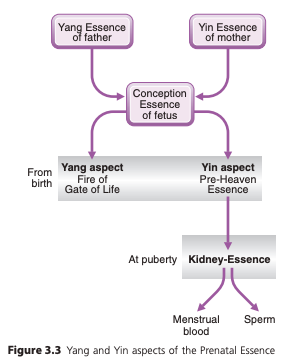
\includegraphics[width=\textwidth]{Images/Yang and Yin aspects of the Prenatal Essence.png}
		\column{0.5\textwidth}
		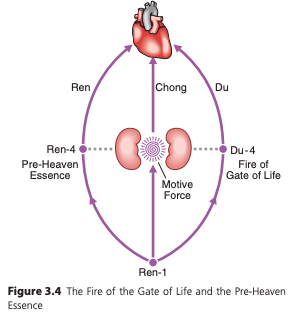
\includegraphics[width=\textwidth]{Images/The Fire of the Gate of Life and the Pre-Heaven Essenc.png}
	\end{columns}
\end{frame}

\begin{frame}{Tinh-ESSENCE}{Tinh hậu thiên - Post-Heaven Essence}
\begin{quote}
	The Pre-Heaven Essence originates from the parents, the Post-Heaven Essence originates from food
\end{quote}
\begin{itemize}
	\item Lungs, Stomach and Spleen start functioning to produce Qi from food, drink and air
	\item The Stomach and Spleen are also known as the Root of the Post-Heaven
	Essence and the Kidneys as the Root of the Pre-Heaven Essence.
\end{itemize}
\end{frame}
\begin{frame}{The Kidney-Essence}
	\begin{itemize}
		\item Unlike the Pre-Heaven Essence, however, the Kidney Essence interacts with the Post-Heaven Essence and is replenished by it.
		Kidney Essence therefore partakes of both the Pre-Heaven and the Post-Heaven Essences.
		\item This Essence is stored in the Kidneys, but it also circulates all over the body, particularly in the Eight Extraordinary Vessels
	\end{itemize}
\end{frame}
\begin{frame}{Some differences between Essence and Qi in the human body}
	\begin{block}{}
		\begin{itemize}
			\item Essence is primarily derived from the parents before birth, 
			whilst Qi is formed after birth
			\item Essence is replenished only with difficulty, Qi can easily be 
			replenished on a day-to-day basis
			\item Essence follows very long cycles of 7 or 8 years, whereas Qi 
			follows briefer cycles, some yearly, some circadian, some 
			even shorter
			\item Qi moves and changes quickly from moment to moment, 
			whereas the Essence changes only slowly and gradually 
			over long periods of time
		\end{itemize}		
	\end{block}
\end{frame}
\begin{frame}[plain]
	\Huge{Thần-Shen}\\
	\Large{Mind or Spirit}\\
	\begin{block}{}
		translate Shen as 'Mind' and use 'Spirit' for the complex of 
Ethereal Soul (Hun), Corporeal Soul (Po), Intellect (Yi), 
Will-power (Zhi) and Mind (Shen) itself
	\end{block}
\end{frame}
\begin{frame}{Thần-SHEN}{Liên quan mật thiết Tạng Tim}
	\begin{columns}
		\column{0.5\textwidth}
		\begin{block}{Thần}
			Là tinh thần, ý thức, tri giác, tư duy, chi phối tất cả hoạt động. Được sinh ra từ tinh tiên thiên và nuôi dưỡng bởi tinh hậu thiên. Thần sung túc cơ thể khỏe mạnh, Thần suy nhược cơ thể yếu đuối.
		\end{block}
		Bao gồm Hồn, Phách, Ý và Trí
		\begin{itemize}
			\item Can tàng Hồn
			\item Phế tàng Phách
			\item Tỳ tàng Ý
			\item Thận tàng Trí
		\end{itemize}
		\column{0.5\textwidth}

	\end{columns}
	
	\small{The Heart is the Monarch of the five Yin organs and six Yang organs and it is the residence of the Mind}
\end{frame}

\begin{frame}{Thần-SHEN}{}
	\begin{columns}[t]
		\column{0.5\textwidth}
		Shen encompasses both the Mind and the Spirit. It reflects the entire physical, emotional, mental and spiritual health of the body. It includes the capacity to think and act coherently, the force of the human personality, and the joy to live. It also includes the spiritual aspects ofall the organs, especially the Yin organs. It is distinguished by the sparkle in the eyes, an overall vivaciousness and the will to live. Shen is housed in the Heart. Because of its active nature, it is a part of Yang.
		\column{0.5\textwidth}

	\end{columns}
\end{frame}
\begin{frame}[plain]
	\begin{columns}[T]
		\column{0.5\textwidth}
		\begin{center}
			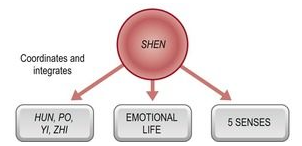
\includegraphics[width=\textwidth]{Images/The coordinating and integrating function of the Mind (Shen ).png}
		\end{center}
		\begin{block}{Chức năng}
			\begin{itemize}
				\item Consciousness (Ý thức)
				\item Thinking (Suy nghĩ)
				\item Memory (Nhớ)
				\item Insight (Minh mẫn)
				\item Cognition (nhận thức)
				\item Sleep (Ngủ)
				\item Intelligence (Trí tuệ)
				\item Wisdom (Trải nghiệm)
				\item Ideas (Ý tưởng)
				\item Affections (Cảm giác)
				\item Feelings (Cảm nhận)
				\item Senses (Giác quan)
			\end{itemize}
		\end{block}
		\column{0.5\textwidth}
		\begin{center}
			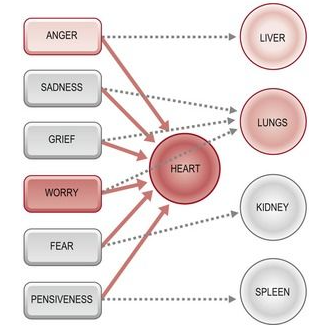
\includegraphics[width=\textwidth]{Images/Affliction of the Heart by all emotions.png}
		\end{center}
	\end{columns}
\end{frame}
\begin{frame}[plain]
	\Huge{Qi-Khí}\\
	\Large {Yuan Qi (Original Qi)- Nguyên khí \\
	Zong Qi (Pectoral/ Ancestral Qi )- Tông khí \\
	Wei Qi (Defensive Qi) - Vệ khí \\
	Ying Qi (Nutritive Qi)- Dinh khí \\
	}

\end{frame}
\begin{frame}{Khí-Qi}{It is a part of Yang and includes motivation and warmth for the body. Qi transforms, transports, holds, protects, raises up and warms.}
	\begin{block}{Chức năng}
		Là thành phần cấu tạo cơ thể. Chất cơ bản duy trì sự sống (khí của thủy cốc, khí hô hấp). Năng lượng hoạt động của các tổ chức (ngũ tạng, lục phủ), Khí của kinh mạch. Có ở khắp cơ thể, có tác dụng chung và riêng ở nơi trú ngụ (thận khí, can khí)
	\end{block}
	\Large{Phân loại theo nguồn gốc}\\
	\normalsize{
	\begin{itemize}
		\item Khí tiên thiên (nguyên khí): Được hình thành từ bào thai, truyền từ cha mẹ, bổ sung bởi khí hậu thiên
		\item Khí hậu thiên: Từ khí trời, khí đồ ăn, nuôi dưỡng khí tiên thiên, cung cấp năng lượng cho hoạt động tạng phủ
	\end{itemize}
	}
	\Large{Phân loại theo chức năng}\\
	\normalsize{
	Nguyên khí, Tông khí, Vị khí, Sinh khí}
\end{frame}

\begin{frame}
	\Huge{THE CLASSIFICATIONS OF Qi}\\
\end{frame}
\begin{frame}{Khí}{Nguyên khí ORIGINAL QI (YUAN QI)}
	\begin{block}{Nguồn gốc}
		Tinh tiên thiên và bổ sung bởi khí hậu thiên bao gồm nguyên dương và nguyên âm.\\
		Bắt nguồn từ Thận, tàng ở Đang điền nhờ Tam tiêu vận hành tuần hoàn cơ thể.
	\end{block}
	\begin{block}{Chức năng}
		Cung cấp năng lượng cho hoạt động của lục phủ ngũ tạng các hoạt động sinh lý cơ thể, điều hoà các hoạt động liên quan đến sinh trưởng, phát triển và sinh dục 
	\end{block}
	Nguyên khí đầy đủ cơ thể khỏe mạnh và ngược lại
\end{frame}
\begin{frame}{Nguyên khí ORIGINAL QI (YUAN QI)}
	\begin{columns}[T]
		\column{0.4\textwidth}
		\begin{block}{}
			It is a dynamic and rarefied form of Essence having its origin in the Kidneys. Original Qi is also often said to include the Original Yin (Yuan Yin) and Original Yang (Yuan Yang): this means that Original Qi is the foundation of all the Yin andYang energies of the body
		\end{block}
		\begin{block}{}
			Original Qi, like Essence, relies on nourishment from the Post-Heaven Essence.
		\end{block}
		\column{0.55\textwidth}
			\only<1>{
				\begin{block}{Motive force}		
Original Qi can be seen as the dynamic motive force
that arouses and moves the functional activity of all
the organs. It does so because, like the Essence, it is the
foundation of vitality and stamina. As a form of Qi, it
circulates all over the body, in the channels. It could be
said to be the link between Essence, which is more fluid like and related to slow, long-term cycles and changes,
and the day-to-day Qi, which is Qi-like and is related to
short-term cycles and changes
				\end{block}
			}
			\only<2>{
				\begin{block}{Basis of Kidney-Qi}		
					
					Original Qi is the basis for Kidney-Qi and is closely
					related to all the Kidneys functional activities. Original
					Qi dwells between the two Kidneys below the umbilicus, at the Gate of Life. Thus, Original Qi is closely related to the Gate of Life and shares its role of providing the heat necessary to	all the bodys functional activities
				\end{block}
			}
			\only<3>{
				\begin{block}{Facilitates the transformation of Qi}				
Original Qi acts as the agent of change in the transformation of Gathering Qi (Zong Qi) intoTrue Qi (Zhen Qi).
This is one way in which the Kidneys (where the Original Qi arises from) participate in the production of Qi
				\end{block}
			}
			\only<4>{
				\begin{block}{Facilitates the transformation of Blood}				
Original Qi acts as the agent of change in the transformation of Gathering Qi (Zong Qi) intoTrue Qi (Zhen Qi).
This is one way in which the Kidneys (where the Original Qi arises from) participate in the production of Qi
				\end{block}
			}
			\only<5>{
				\begin{block}{Facilitates the transformation of Blood}				
Original Qi acts as the agent of change in the transformation of Gathering Qi (Zong Qi) intoTrue Qi (Zhen Qi).
This is one way in which the Kidneys (where the Original Qi arises from) participate in the production of Qi
				\end{block}
			}
			\only<6>{
				\begin{block}{}
					\begin{enumerate}
						\item Is the Motive Force of all physiological activities
						\item Is the basis of Kidney-Qi
						\item Helps transformation of Gathering Qi (Zong Qi) into True Qi (Zhen Qi)
						\item Helps transformation of Food-Qi (Gu Qi) into Blood
						\item Comes out at the Source (Yuan) point
					\end{enumerate}
				\end{block}
			}
	\end{columns}
\end{frame}
\begin{frame}{Khí}{Tông khí-GATHERING QI (ZONG QI)}
	\begin{block}{Nguồn gốc}
		Từ hai nguồn là cốc khí (food) sau khi tỳ vị vận hóa thủy cốc (water)cộng thêm khí trời (phổi) (air) tạo tông khí tích tụ ở ngực
	\end{block}
	\begin{block}{Chức năng}
		\begin{itemize}
			\item Từ phế theo đường hô hấp và hầu họng để thực hiện hô hấp. Vào tâm mạch để vận hành khí huyết.
			\item Đi xuống dưới qua tam tiêu vào đan điền.
			\item Từ đan điền, khí vận hành tuần hoàn toàn thân.
		\end{itemize}

	\end{block}
\end{frame}
\begin{frame}{Khí}{Dinh khí- NUTRITIVE QI (YING QI)}
	\begin{block}{Nguồn gốc}
		Từ thủy cốc 
	\end{block}
	\begin{block}{Chức năng}
		Vi hành trong mạch, sinh hóa huyết-dịch\\
		Công năng dinh dưỡng toàn thân, lục phủ ngũ tạng phát tán ra ngoài nuôi dưỡng da lông\\
		Dinh khí vào trung tiêu, tàng tại thủ thái âm phế kinh tuần hoàn 14 đường kinh vận hành liên tục.
	\end{block}
\end{frame}
\begin{frame}{Dinh khí- NUTRITIVE QI (YING QI)}
	\begin{columns}
		\column{0.4\textwidth}
		\begin{block}{}
			Nutritive Qi is extracted from food and water, it regulates the 5 Yin organs, moistens the 6 Yang organs, it enters the blood vessels, it circulates in the channels above and below, is linked with the 5 Yin organs and connects with the 6 Yang organs
		\end{block}
		\column{0.55\textwidth}
		\begin{block}{}
			\begin{enumerate}
				\item Nourishes the Internal Organs
				\item Is closely linked to Blood
				\item Flows in channels and blood vessel
			\end{enumerate}
		\end{block}
	\end{columns}
\end{frame}

\begin{frame}{Khí}{Tông khí-GATHERING QI (ZONG QI)}
	\begin{columns}[T]
		\column{0.4\textwidth}
		\begin{block}{}
		the Gathering Qi derives from the interaction of Food-Qi with air. The Spleen sends Food-Qi up to the Lungs where, combining with air, it is transformed into Gathering Qi
		\end{block}
		\begin{block}{}
			Gathering Qi is a more subtle and refined form of Qi than Food-Qi, and it is usable by the body.
		\end{block}
		\column{0.55\textwidth}
		\only<1>{
			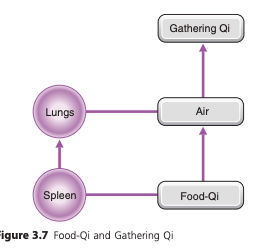
\includegraphics[width=\textwidth]{Images/Food-Qi and Gathering Qi.png}}
		\only<2>{
			\begin{block}{}
				\begin{enumerate}
					\item It nourishes Heart and Lungs
					\item It enhances and promotes the Lung function of controlling Qi and respiration, and the Heart function of governing Blood and blood vessels
					\item It controls the speech and the strength of voice
					\item It affects and promotes blood circulation to extremities
					\item It is coordinated with Original Qi to regulate breathing
				\end{enumerate}
			\end{block}

		}
	\end{columns}
\end{frame}

\begin{frame}{Vệ khí- DEFENSIVE QI (WEI QI)}
	\begin{block}{Nguồn gốc}
		Từ thủy cốc
	\end{block}
	\begin{block}{Chức năng}
		Bắt nguồn từ Tỳ, Vị; vận hành ngoài Mạch. Bên trong phân bố ở các màng có màu đen ở ngực bụng, ngoài tuần hoàn giữa cơ nhục và bì phu.\\
Vệ khí vào thượng tiêu, công năng ôn dưỡng cơ nhục bì phu (làm ấm nội tạng, cơ nhục, da lông, đóng mở tấu lý (lỗ chân lông). Bảo vệ cơ thể chống ngoại tà xâm nhập.
	\end{block}
\end{frame}
\begin{frame}{Vệ khí Defensive Qi (Wei Qi)}
	\begin{columns}[T]
		\column{0.4\textwidth}
		\begin{block}{}
			The human 
being receives Qi from food: this enters the stomach, is 
transported to the Lungs [i.e. the Food-Qi] it is transformed into Qi, the refined part becomes Nutritive Qi, the 
coarse part becomes Defensive Qi. Nutritive Qi flows in 
the blood vessels [and channels], Defensive Qi flows outside 
the channels.
		\end{block}
		\begin{block}{}
			Defensive 
Qi is derived from the coarse part of food and water, it is 
slippery in nature, hence it cannot enter the channels. It 
therefore circulates under the skin, in between the muscles, 
it vapourizes in between membranes and diffuses over the 
chest and abdomen
		\end{block}
		\column{0.55\textwidth}
		\only<1>{
			\begin{block}{}
				\begin{itemize}
					\item Nutritive Qi is in the Interior and nourishes
					\item Defensive Qi is on the Exterior and protects
				\end{itemize}
			\end{block}
			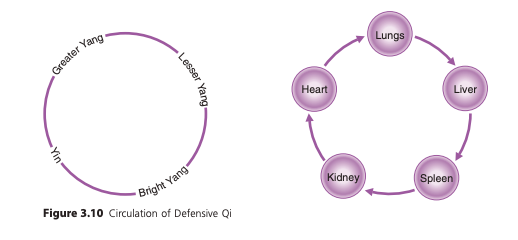
\includegraphics[width=\textwidth]{Images/Circulation of Defensive Q.png}
		}
		\only<2>{
			\begin{block}{}
				\begin{itemize}
					\item Has its root in the Lower Burner (Kidneys), it is nourished by the Middle Burner (Stomach and Spleen), and it spreads outwards in the Upper Burner (Lungs)
					\item It is a coarse form of Qi
					\item It circulates outside the channels in the space between skin and muscles
					\item It protects the body from invasion of external pathogenic 
					factors
					\item It warms the muscles
					\item It is mixed with sweat in the space between skin and 
					muscles and it regulates the opening and closing of pores
					\item It circulates 50 times in 24 hours: 25 during the day and 25 at nigh
				\end{itemize}	
			\end{block}
		}
	\end{columns}
\end{frame}
\begin{frame}{Một số loại khí khác}
	\begin{itemize}
		\item Central Qi (Zhong Qi)
		\item Upright Qi (Zheng Qi) 
		\item True Qi (Zhen Qi)
		\item Food-Qi (Gu Qi) 
	\end{itemize}
\end{frame}
\begin{frame}
	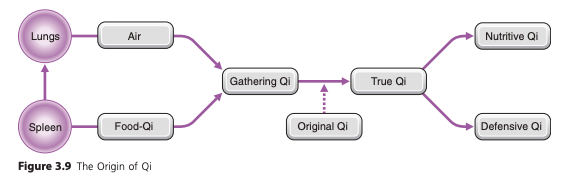
\includegraphics[width=\textwidth]{Images/The Origin of Qi.png}
\end{frame}
\begin{frame}
	\Huge{Functions of Qi}\\
\end{frame}
\begin{frame}{Functions of Qi}
	\begin{columns}[T]
		\column{0.25\textwidth}
		\begin{itemize}
			\item Transforming
			\item Transporting
			\item Holding
			\item Raising
			\item Protecting
			\item Warming
		\end{itemize}
		\column{0.65\textwidth}
		\only<1>{
			\begin{block}{Transforming}
				\small{Qi (Yang in nature) is essential for the transformation
				of food and fluids (Yin in nature) into clear (Yang) and
				turbid (Yin) parts. This process of transformation is
				anotheraspectof thechangeinthestateof aggregation/
				dispersion of Qi mentioned above. Material, dense
				forms of matter such as food and fluids need the power
				of Qi to be transformed into more subtle forms of
				matter, e.g. food is transformed into Food-Qi which is,
				in turn, transformed into True Qi}
			\end{block}
		}
		\only<2>{
			\begin{block}{Transporting}
				\small{Transportation, closely linked to transformation, is
				another essential function of Qi. In the process of
				transformation of various substances, Qi transports
				them in and out of various body structures. This transportation movement may be upwards, downwards,inwards or outwards. The ascending/descending and entering/exiting of Qi in the body constitutes what is	called the Qi Mechanism (Qi Ji)}
			\end{block}
		}
		\only<3>{
			\begin{block}{Holding}
				\small{Holding means that Qi (Yang in nature) holds fluids
				and Blood (Yin in nature) in their proper places. This is
				essential so that fluids or blood do not leak out.}
			\end{block}
		}
		\only<4>{
			\begin{block}{raising}
				\small{Qi ensures that the body structures are held in their
				proper place. If Qi is deficient, particularly in its raising
				function, it is said to be not only deficient but also
				sinking}
			\end{block}
		}
		\only<5>{
			\begin{block}{Protecting}
				\small{Qi protects the body from invasion of exterior pathogenic factors. This is primarily (but not exclusively) a
				function of Defensive Qi. Defensive Qi irrigates the
				space between the skin and muscles which constitutes
				the exterior energetic layer of the body. The strength of
				Defensive Qi in this space determines our resistance to
				external pathogenic factors such as Wind, Cold and
				Dampness. Defensive Qi is closely linked to the Lungs
				which spread it in the space between skin and muscles
				and therefore Lung-Qi protects the body from exterior
				pathogenic factors.
				However, our overall resistance to external pathogenic factors does not depend only on the strength of
				Defensive Qi but partly also on that of Nutritive Qi and
				Kidney-Essenc}
			\end{block}
		}
		\only<6>{
			\begin{block}{Warming}
				\small{This is a function of Yang-Qi. Warming is an essential
				role for Qi as all physiological processes depend on
				warmth: this is especially crucial with fluids, as they
				are Yin in nature and therefore need Yang (warmth)
				to promote their transformation, transportation and
				excretion.
				The source of Yang and warmth in the body is primarily Kidney-Yang and the Minister Fire. Spleen Yang also warms the body but it, in turn, derives its
				warmth primarily from Kidney-Yang.}
			\end{block}
		}
	\end{columns}
\end{frame}
\begin{frame}[plain]
	\Huge{Direction of Qi movement}\\
	\normalsize{
	\begin{quote}
		Without exiting-entering of Qi, there  would be no birth, growth, maturity and decline. Without ascending-descending, there would be no birth, growth, transformation, receiving and storage. All organs rely on the ascending-descending and exiting-entering of Qi.
	\end{quote}
	}
\end{frame}
\begin{frame}
		\begin{block}{Qi Mechanism}
			\begin{enumerate}
				\only<1>{
				\item Qi Mechanism indicates the flow of Qi in all organs of the 
				body, all Triple Burner cavities, joints, skin, muscles, 
				diaphragm, Fat Tissue, Membranes
				\item The movement of Qi in the Qi Mechanism comprises the 
				ascending-descending and entering-exiting of Qi in every 
				part of the body
				\item The Qi Mechanism is like a vast system of roads and 
				motorways (freeways) where traffic needs to be regulated 
				by one-way streets
				\item The smooth movement of Qi in the Qi Mechanism relies on 
				the proper ascending and descending of Qi in various 
				organs and structures and also on the entering and exiting 
				of Qi in and out of various structures
				}
				\only<2>{
				\item The balance of Yin and Yang is crucial for the smooth 
				movement of Qi, as ascending and exiting are Yang 
				movements while descending and entering are Yin 
				movements
				\item An excess of Yang will imply excessive ascending and 
				exiting of Qi, while an excess of Yin will imply excessive 
				descending and entering of Qi
				\item When the Qi Mechanism is disrupted, there will be Qi 
				stagnation or Qi rebelliou
				}
			\end{enumerate}
		\end{block}
\end{frame}
\begin{frame}
	\begin{center}
		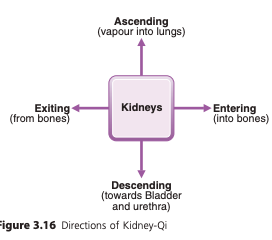
\includegraphics[width=0.3\textwidth]{Images/Directions of Kidney-Qi.png}
		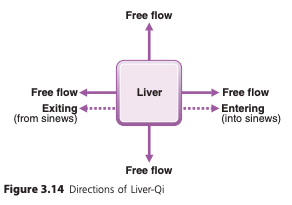
\includegraphics[width=0.3\textwidth]{Images/Directions of Liver-Qi.png}
		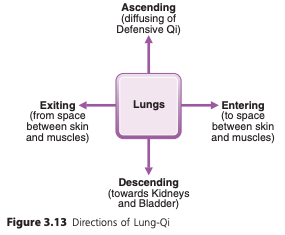
\includegraphics[width=0.3\textwidth]{Images/Directions of Lung-Qi.png}
	\end{center}

\end{frame}
\begin{frame}{Quan niệm Qi}{Chinese Traditional Herbal Medicine}
	\begin{quote}
		Just as science has discovered that the DNA molecule is the all- pervasive code of life manifesting as different tissues and organs throughout the body, Qi, which is essentially one, manifests in different forms and qualities depending upon its functions within the body. In TCM, Qi has two major aspects in the body. In one, it represents a refined aspect, or Essence, which nourishes the body-mind complex. This Essence is expressed in different forms according to its location and function in the body. In its second aspect, Qi indicates the functional activities of the internal organs themselves.
	\end{quote}
\end{frame}

\begin{frame}{Các cách tiếp cận về Qi}{Liệu Qi có phải là một Pseudoscientific}
	\only<1>{
	\begin{block}{Góc nhìn khoa học}
		\begin{itemize}
			\item Hiện tại chưa có bằng chứng về tồn tại của QI.
			\item Năm 1998, Viện Y tế quốc gia Hoa kỳ đã có sự đồng thuận liên quan đến châm cứu với lưu ý rất khó để dung hòa Qi với thông tin y sinh đương thời. 
		\end{itemize}
	
	\end{block}
	}
	\only<2>{
		\begin{block}{The idealist view}
			\begin{enumerate}
				\item {\bf Epistemological-Thuyết bất khả tri}: Chủ thể khách quan có thể tồn tại nhưng chúng ta sẽ không bao giờ tiếp cận được. Quan niệm của chúng ta chỉ là thực tế chủ quan.
				\item {\bf Ontological-Thuyết duy tâm bản thể luận}: Thế giới vật chất không thực tế tồn tại và mọi thứ đơn thuần chỉ là ý tưởng và cấu trúc chủ quan của tâm trí.
			\end{enumerate}
		\end{block}
		}
		\only<3>{
		\begin{block}{Cách tiếp cận lấy bệnh nhân làm trung tâm}
			\begin{enumerate}
				\item Phương pháp nghiên cứu hiện đại rốt cuộc cốt lõi đem lại tiến bộ trong chăm sóc sức khỏe.
				\item Cần thận trọng áp dụng phương pháp cổ truyền khi luôn cân nhắc giữa lợi ích và nguy cơ.
				\item Liệu Qi có phải là hiệu quả của phương pháp giả dược cần phải được cân nhắc và khai thác một cách khôn ngoan. Mặc dù, theo quan niệm chính thống từ Descartes cho rằng tâm trí không tác động được đến thể chất.
			\end{enumerate}
		\end{block}
		}
	\vspace{\fill}
	\tiny{The idealist and pragmatist view of qi in tai chi and qigong: A narrative commentary and review, George Chengxi Bao, 2020}
\end{frame}
\begin{frame}
	\Huge{Huyết-BLOOD}
\end{frame}
\begin{frame}{Huyết-BLOOD}{a part of Yin, The concept of Blood is similar, though broader in definition to, Western medicine and includes circulation, stagnation and hemorrhage.}
	\begin{block}{Nguồn gốc}
		Vật chất sắc đỏ, tạo thành từ tinh của thủy cốc và tinh thận thông quá trình khí hòa nhờ chức năng của tỳ, vị, tâm, phế và thận
	\end{block}
	\begin{block}{Chức năng của huyết}
		\begin{itemize}
			\item Huyết chứa chất dinh dưỡng, vận hành trong mạch, đi nuôi dưỡng toàn thân
			\item Huyết thiếu, huyết hư: Tê mỏi bộ phận; 
			\item Huyết tắc, Huyết ứ : tê liệt bộ phận
			\item Khí, Huyết đầy đủ: Tinh thần minh mẫn, vui vẻ sảng khoái, khỏe khoắn
		\end{itemize}
	\end{block}

\end{frame}
\begin{frame}
	\begin{columns}
		\column{0.6\textwidth}
		\small{
		\begin{itemize}
			\item The Spleen and Stomach are the main source of Blood
			\item Lung-Qi plays an important role in pushing Food-Qi to the 
			Heart: this is an example of the general principle that Qi 
			makes Blood move
			\item Food-Qi is transformed into Blood in the Heart: this is one 
			aspect of the principle that the Heart governs Blood
		\end{itemize}
		}
		\column{0.4\textwidth}
		\small{
			\begin{quote}
				If Qi is not exhausted, it returns essences to the Kidneys to be transformed into Essence; if the Essence is not depleted, it returns Essence to the Liver to be transformed into Blood.
			\end{quote}

		}
	\end{columns}
	\begin{center}
		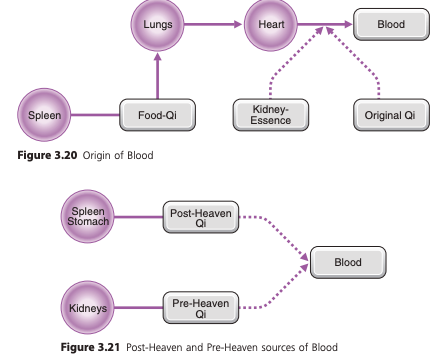
\includegraphics[width=0.5\textwidth]{Images/Origin of Blood.png}
	\end{center}
\end{frame}
\begin{frame}{Relation of Blood with internal organs}
	\includegraphics[width=0.5\textwidth]{Images/Relationship of Heart, Spleen and Liver with Blood.png}
	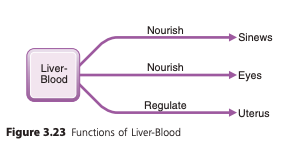
\includegraphics[width=0.5\textwidth]{Images/Functions of Liver-Blood.png}
\end{frame}
\begin{frame}{Blood Qi relationship}
	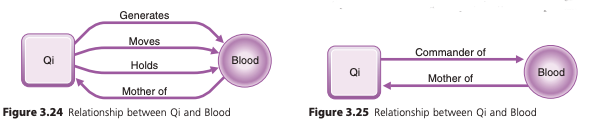
\includegraphics[width=\textwidth]{Images/Qi and Blood.png}
\end{frame}
\begin{frame}{Tân dịch-Body Fluids}{a part of Yin. Fluids describe all the various fluidic substances including saliva, sweat, urine, tears, lymph and other secretions.}
	Tân dịch là tất cả các dịch trong cơ thể bao gồm cả dịch trong tạng phủ trừ tinh và huyết.\\
	Tân dịch có nguồn gốc từ thủy cốc\\
	Tân loãng, nhẹ như tấu lý (mồ hôi), bàng quang (nước tiểu): Ôn dưỡng cơ nhục nhuận da lông\\
	Dịch đặc nhớt như dịch não, tủy, nhuận khớp, nhuận tạng bổ não tủy\\
	Tân dịch không dùng hết dư thừa sẽ đi vào mạch. Dịch trong cơ thể ở trạng thái cân bằng. 
\end{frame}
\begin{frame}
	\includegraphics[width=\textwidth]{Images/Origin, transformation and excretion of Body Fluids.png}
\end{frame}
\begin{frame}
	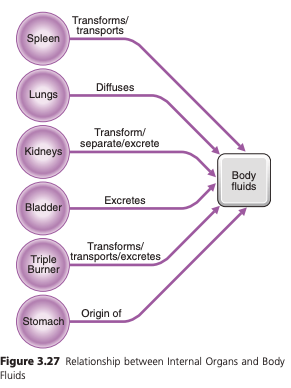
\includegraphics[width=0.6\textwidth]{Images/Relationship between Internal Organs and Body Fluids.png}
\end{frame}
\section{Học thuyết tạng tượng \newline  Zang-xiang theory}
\begin{frame}[plain]
	\Huge{}
\end{frame}
\begin{frame}{Khái niệm chung}
	\begin{block}{Học thuyết tạng tượng}
		Nghiên cứu về kết cấu hình thái, quy luật hoạt động sinh lý và quá trình biến hóa bệnh lý của cơ quan, tổ chức tạng phủ trong cơ thể; là quy luật hoạt động của các bộ phận trong cơ thể theo nguyên lý của y học cổ truyền 
	\end{block}
	\begin{block}{Theory of zang-fu organs}
		The theory of zang-fu organs discusses the physiological functions and pathological changes of the zang-fu organs as well as their relationships with each other.
	\end{block}
	\small{
		\begin{itemize}
			\item {\bf Tạng:} là các cơ quan trong cơ thể.
			\item {\bf Tượng:} Biểu hiện hình thái, sinh lý, bệnh lý của nội tạng phản ánh bên ngoài cơ thể.
			\item Tạng có tên gọi trùng giải phẫu của phương tây nhưng khác biết về cách tiếp cận.
		\end{itemize}
	}
\end{frame}
\begin{frame}{Khái niệm chung}
	\begin{itemize}
		\item Cấu tạo theo đông y
		\begin{itemize}
			\item {\bf Ngũ tạng:} Tâm, Can, Tỳ (Lách), Phế, Thận 
			\item {\bf Lục phủ:} Tiểu Tràng, Đại Tràng, Bàng Quang, Tam Tiêu, Vị, Đởm
			\item {\bf Phủ kỳ hằng:} Não, Tủy, Mạch, Tử cung
			\item {\bf Các thành phần khác:} Cơ nhục, tứ chi, cân cốt, Tinh, Khí, Thần, Huyết, Tân Dịch
		\end{itemize}
		\item Vai trò chức năng
		\begin{itemize}
			\item Tạng: Hóa sinh và tàng trữ vật chất tinh:  Tinh Khí (Tinh, Khí, Huyết và Tân Dịch) để duy trì hoạt động sống phức tạp của cơ thể
			\item Phủ: Thu nạp và chuyển hóa thủy cốc sinh ra tinh khí. Tinh khí có sẽ được chuyển đến các tạng, còn phủ chỉ bài xuất mà không tàng trữ lại bên trong
			\item Phủ kỳ hằng: Hình thái, kết cấu của phủ kỳ hằng phần lớn là rỗng như phủ nhưng công năng lại là tàng trữ tinh khí giống như tạng
		\end{itemize}
	\end{itemize}
\end{frame}

\begin{frame}{Khái niệm chung}
	\begin{block}{Zang-xiang}
		The word zang means the internal organs; and the word xiang means the outward manifestations of physiological functions and pathological changes of the internal organs. 
	\end{block}
	\begin{block}{Zang fu}
		A collective term for the internal organs of human beings, including five zang organs, six fu organs and extraordinary organs.
		\begin{itemize}
			\item Five zang organs: A collective term for the five internal organs—the heart, liver, spleen/pancreas, lung and kidney.
			\item Six fu organs: A collective term for the six internal organs: 
			gallbladder, stomach, large intestine, small intestine, urinary bladder, and sanjiao (literally translated into triple energizer).
			\item Extraordinary fu organs: A collective term for brain, marrow, bone, vessels, gallbladder and uterus. These organs are 
			extraordinary because they store like zang organs. 
		\end{itemize}
	\end{block}
\end{frame}
\begin{frame}{Các thuật ngữ}
	\only<1>{
		\begin{block}{Zang-fu organs mutually interconnect}
			The zang-fu organs mutually correspond with one another, with a (yin) interior-(yang) exterior connection between the zang and fu organs. Specifically, the heart is internally-externally connected with the small intestine, the lung with the large intestine, the spleen with the stomach, the liver with the gallbladder, the kidney with the urinary bladder, and the pericardium with sanjiao.
		\end{block}
	}
	\only<2>{
		\begin{block}{Storage of the five zang organs}
			The heart stores the spirit; the lung stores the corporeal soul; the liver stores the ethereal soul; the spleen stores the intent; and the kidney stores the will. 
		\end{block}
	}
	\only<3>{
		\begin{block}{Governance of the five zang organs }
			The heart governs blood vessels; the lung governs the skin; the spleen governs the flesh; the liver governs the sinew/tendon; and the kidney governs the bones. 
		\end{block}
	}
	\only<4>{
		\begin{block}{Fluids of the five zang organs}
			The fluid of the heart is sweat; the fluid of the lung is nasal mucus; the fluid of the spleen is thin saliva; the fluid of the liver is tears; and the fluid of the kidney is the thick saliva. 
		\end{block}
	}
	\only<5>{
		\begin{block}{Lustres of the five zang organs}
			The lustre of the heart shows in the face; the lustre of the lung shows in the skin hair; the lustre of the spleen shows in the lips; the lustre of the liver shows in the nails; and the lustre of the kidney shows in the hair. 
		\end{block}
	}
	\only<6>{
		\begin{block}{Opening of the five zang organs}
			The heart opens into the tongue; the lung opens into the nose; the spleen opens into the mouth; the liver opens into the eyes; and the kidney opens into the ears. 
		\end{block}
	}
	\only<7>{
		\begin{block}{Emotions of the five zang organs}
			The emotion of the heart is joy; the emotion of the lung is grief; the emotion of the spleen is overthinking; the emotion of the liver is anger; and the emotion of the kidney is fear. 
		\end{block}
	}
	\only<8>{
		\begin{block}{Dislikes of the five zang organs}
			The heart dislikes heat; the lung dislikes cold; the spleen dislikes dampness; the liver dislikes wind; and the kidney dislikes dryness. 
		\end{block}
	}

\end{frame}

\begin{frame}
	\Huge{Tạng Tâm}
\end{frame}

\begin{frame}{Tạng Tâm}{Là quân hỏa, trung tâm hoạt động sống của cơ thể}
{\bf Đặc điểm:} Hành Hỏa, mùi khét, màu đỏ, vị đắng, nóng nhiệt, tiếng cười, vui mừng; liên quan đến giấc mơ và nói chuyện\\
{\bf Chức năng sinh lý}\\
\begin{itemize}
	\only<1>{
	\item Tâm chủ huyết mạch (tâm quản lý về huyết mạch): Tốt mặt hồng nhuận sáng sủa, da dẻ tươi nhuận. Kém  mặt xanh xao, xám héo, môi thâm  Thuốc hành huyết, hành khí, bổ huyết, bổ âm.
	\item Tâm tàng Thần (chủ Thần chí): Tốt  Thông minh, hoạt huyết; kém  hay quên, tư duy kém, mất ngủ, mệt mỏi. Liên quan Tâm chủ Huyết. 
	\item Thần biểu hiện ra mắt: Tốt  mắt trong sáng tinh tường, kém  mắt lờ đờ, chậm chạp  Thuốc trấn tâm an thần, gây ngủ, bổ huyết, bổ âm, khai khiếu tỉnh thần}
	\only<2>{
	\item Tâm chủ Hãn (mồ hôi sản phẩm thanh lọc của chất Tân). Bệnh tự hãn, đạo hãn, vô hãn, liên quan tàng thần. Không tàng được thần  mồ hôi tự vã (việc kinh khủng, trúng phong, trúng thử, Thần hôn mê)  Thuốc liễm hãn, cố biểu, an thần
	\item Tâm hợp mạch, vinh nhuận ra mặt, khai khiếu ra lưỡi: Thể chất lưỡi, màu sắc thể hiện tình trạng Tâm. Tốt: hồng, mềm mại; nhợt nhạt, cứng, lệch, ngọng, không nói}
\end{itemize}
\end{frame}

\begin{frame}{Tạng tâm}{Bệnh lý của tạng Tâm}
	\begin{itemize}
		\item Tâm dương hư: Tim đập nhanh (tâm quý), khí đoản (hơi thở ngắn), khó thở, trắng bệch, lưỡi nhợt nhạt, môi tím tái, sợ lạnh, hoa mắt, chóng mặt, mạch vi tế dưỡng tâm an thần, hóa đờm, bổ khí, bổ huyết
		\item Tâm huyết bất túc: Huyết thiếu, tim đập nhanh, hay quên, mất ngủ, mộng, da xanh xao, lưỡi trắng nhợt, thân nhiệt hạ  bổ huyết, an thần
		\item Tâm huyết ứ trệ: đau vùng tim, tim đạp nhanh, mặt môi móng tay thâm    hành khí, hành huyết
		\item Tâm hỏa vượng: mặt đỏ, miệng đắng, niêm mạc miệng lưỡi phồng rộp, đầu lưỡi đỏ, tiểu tiện nóng đỏ, lòng tay chân nóng  thanh nhiệt, lợi thủy, an thần
	\end{itemize}
\end{frame}

\begin{frame}
	\Huge{Tạng Can}
\end{frame}

\begin{frame}{Tạng Can}{Hành Mộc, mùi tanh, màu xanh, vị chua, gió, la hét, giận dữ, nước mắt}
Chức năng sinh lý:
\begin{itemize}
	\only<1>{
	\item Can chủ sơ tiết: Sơ tiết mật. Tốt  Tiêu hóa tỳ vị tốt. Kém  đầy bụng, không tiêu, hoàng đản (vàng da), đầy tức, bế kinh, rối loạn kinh nguyệt.  Thuốc sơ can giải uất, hành khí, hành huyết, lợi mật
	\item Can tàng Huyết: Hoạt động  Huyết từ Can đến toàn bộ tế bào; nghỉ ngơi, ngủ  tàng tại Can. Không tốt  Bồn chồn, khó ngủ. Tốt Khỏe mạnh hồng hào; kém  cơ thể xanh xao, mệt mỏi, mắt trắng dã  Thuốc bổ huyết, bổ âm, hoạt huyết hành khí
	\item Can chủ Cân (bao cơ, khớp, dây chằng): Kém  co duỗi khó, dây chằng giãn, đi lại khó khăn, trẻ em chậm biết đi hoặc không đi được  Bổ can thận, can huyết
	}
	\only<2>{
	\item Can chủ nộ: tức giận, nóng nảy, cáu gắt hại Can, liên quan đến chức năng chủ sơ tiết, tàng hồn. Không chủ được  sơ tiết kém, ảnh hưởng hoạt động tinh thần, ngủ không yên   Thuốc an thần gây ngủ, bình can, sơ can giải uất
	\item Can hợp cân, vinh nhuận ra móng, khai khiếu ra mắt: Tốt    thị lực tốt. Kém    mắt mờ, thị lực giảm. Đỏ    can hỏa, vàng    can nhiệt, trắng dã    can huyết hư
	}
\end{itemize}
\end{frame}
\begin{frame}{Tạng can}{Bệnh lý}
\begin{itemize}
	\item Can khí uất kết: đau sườn, đau lồng ngực  bụng, kinh nguyệt không đều    sơ can, giải uất, hành khí, hành huyết
	\item Can đởm thấp nhiệt: da vàng, tiểu tiện vàng đỏ, sườn đau căng    thanh nhiệt táo thấp, giải độc, lợi thấp
	\item Can phong nội động: ngã đột ngột, hôn mê bất tỉnh, miệng méo xệch, động kinh    bình can tắt phong, trọng trấn an thần, sơ can giải uất
	\item Can hỏa thượng viêm: đau đầu, mắt đỏ, mặt đỏ, miệng đắng, chảy máu cam    thanh nhiệt giải biểu nhiệt, chỉ huyết
\end{itemize}
\end{frame}
\begin{frame}
	\Huge{Tạng Tỳ}
\end{frame}
\begin{frame}{Tạng tỳ}{Hành Thổ, mùi thơm, màu vàng, vị ngọt, thấp/ ẩm, suy tư, nước bọt}
{\bf Chức năng sinh lý}\\
\begin{itemize}
	\item Tỳ chủ vận hóa (chuyển vận và tiêu hóa thủy cốc, thủy dịch): Tốt    dinh dưỡng cơ thể tốt, thủy dịch điều hòa, kém    dinh dưỡng thiếu, phù nề bụng thiếu albumin, tiết tả
	\item Tỳ ích khí sinh huyết: Tốt    khí dồi dào, cơ thể khỏe mạch. Kém    mệt mỏi đoản hơi, vô lực, da xanh xao
	\item Tỳ khí chủ thăng (lên thượng tiêu) = Tỳ chủ thăng thanh: đưa cốc khí lên Tâm Phế; giữ cho phủ tạng ở vị trí tự nhiên. Tỳ khí hư    chứng sa giáng
	\item Tỳ chủ nhiếp huyết, thống huyết: Tốt    Huyết lưu thông lòng mạch. Không tốt    huyết loạn, tràn lòng mạch (xuất huyết)
	\item Tỳ chủ cơ nhục, tứ chi: Tốt    béo tốt, hồng nhuận; Kém    còi xương, cơ nhục teo nhẽo, chậm biết đi, suy dinh dưỡng
	\item Tỳ vinh nhuận ra môi, khai khiếu ra miệng: Khỏe  muốn ăn, ăn ngon, tiêu hóa tốt. Kém chán ăn, ăn không ngon
\end{itemize}
\end{frame}
\begin{frame}{Tạng Tỳ}{Bệnh lý}
\begin{itemize}
	\item Tỳ khí hư nhược: kém ăn, hấp thu kém, gầy yếu, da xanh, đại tiện lỏng, bụng chướng đầy, sa giáng  kiện tỳ, ích khí, hành khí, tiêu đạo
	\item Tỳ dương hư: ăn kém, bụng sôi, chướng, đại tiện lỏng, co quắp, phù thũng  kiện tỳ, bổ Dương + hóa thấp
	\item Tỳ thấp nhiệt: vàng da, bụng chướng, kém ăn, đại tiện táo kết	thanh nhiệt, táo thấp, lợi thủy, nhuận tràng
	\item Hàn thấp khuẩn tỳ: bụng ngực đầy, toán than mệt mỏi, đại tiện lỏng  hóa thấp + hành khí
\end{itemize}
\end{frame}
\begin{frame}
	\Huge{Tạng Phế}
\end{frame}
\begin{frame}{Tạng phế}{Hành Kim, mùi hôi, màu trắng, vị cay, khí hậu táo, ưu tư, nước mũi}
{\bf Chức năng sinh lý}
\begin{itemize}
	\only<1>{
	\item Phế chủ khí, chủ hô hấp
	\begin{itemize}
		\item Chủ khí: Tham gia tạo ra tông khí; điều tiết sự vận hành thăng giáng của khí thông qua hô hấp
		\item Chủ hô hấp: Vận hành xuất nhập của khí, giúp trao đổi với môi trường, hít thanh thở trọc
	\end{itemize}
	}
	\only<2>{
	\item Phế chủ tuyên phát (hướng lên trên, tán ra ngoài), túc giáng (làm thanh sạch, đi xuống)
	\item Thông qua khí hóa của Phế bài xuất trọc khí của cơ thể
	Trợ Tỳ chuyển Tân Dịch và chất tinh vi của thủy cốc đến toàn thân (Tạng Phủ,...), ra bì mao
	\item Tuyên phát Vệ Khí, điều tiết tấu lý đóng mở, bài xuất mồ hôi. Giúp thông điều thủy đạo   vấn đề: tức ngực, ho, suyễn tức, nghẹt mũi, không ra mồ hôi,...
	}
	\only<3>{
	\item Phế thông điều thủy đạo: Thông qua tuyên phát đưa tân dịch và tinh vi thủy cốc đến toàn thân, đóng mở tấu lý, bài xuất mồ hôi. Thông qua túc giáng đưa thanh khí đến thận và tân dịch đến Bàng Quang hình thành nước tiểu. Chủ nguồn nước trên. Kém   phù
	\item Phế trợ tâm, chủ việc trị tiết: Quản lý hoạt động của các tạng phủ theo quy luật, giúp Tâm tàng thần
	\item Phế hợp bì mao: Đóng mở tấu lý
	\item Phế khí chủ thanh: Tốt   tiếng nói khỏe, kém   trầm khàn, không ra tiếng.
	\item Phế khai khiếu ra mũi: Tốt   thở nhịp nhàng, nhiệt   mũi nóng đỏ, tắc   phập phồng, hư   nắng, cánh mũi xẹp, hay thở dài.
	}
\end{itemize}
\end{frame}
\begin{frame}{Tạng phế}{Bệnh lý}
\begin{itemize}
	\item Phong tà nhập phế: Sợ lạnh, sốt cao, đau đầu, ho, sổ mũi, đau toàn thân   giải biểu + chỉ khái
	\item Phế âm hư: Ho, ít đờm, có tia máu, lưỡng quyền hồng, sốt về chiều, nóng âm ỉ trong xương   bổ âm, chỉ ho, hóa đờm, chỉ huyết
	\item Đờm phế thấp nhiệt: ho, đờm đặc vàng, mùi hôi, đau ngực, sốt   hóa đờm hàn, chỉ khái, bình suyễn, thanh nhiệt
	\item Khí phế hư: ho nhiều, đờm nhiều loãng, đoản hơi, nhiều mồ hôi, tiếng yếu, mệt mỏi  bổ khí, chỉ khái, hóa đờm, cố biểu liễm hãn
\end{itemize}
\end{frame}
\begin{frame}
	\Huge{Tạng thận}
\end{frame}

\begin{frame}{Tạng thận}{ Hành Thủy, mùi thối, màu đen, vị mặn, khí hậu hàn}
{\bf Chức năng sinh lý}\\
\begin{itemize}
	\only<1>{
	\item Thận tàng tinh, chủ sinh dục, phát dục của cơ thể. Thận là gốc tiên thiên, nguồn gốc của sự sống (tiên thiên chi bản, sinh khí chi nguyên): rối loạn chức năng này có liên quan đến những bệnh có tính di truyền, những bệnh bẩm sinh
	}
	\only<2>{
	\item Tinh hậu thiên: Từ chất tinh hoa của đồ ăn uống tạo thành để nuôi dưỡng cơ thể, còn thừa bổ sung cho tinh tiên thiên và tàng trữ ở thận
	Vậy tinh tàng trữ ở thận gồm (tinh tiên thiên và hậu thiên) quyết định sự sinh dục, phát dục của cơ thể từ nhỏ đến trưởng thành sinh con cái đến lúc già. Thúc đẩy sự sinh trưởng, phát dục, sinh đẻ: quy luật nam 8 nữ 7. Nữ 7 tuổi thiên qui thịnh, 14 thiên qui đến, 49 thiên qui suy cạn. Nam 8 tuổi thiên qui thịnh, 16 thiên qui đến, 64 tuổi (8x8) thiên qui suy Quá trình sinh trưởng và phát triển của cơ thể, sinh con cái đều liên quan đến thận tinh, chức năng tàng tinh tốt, cơ thể phát triển tốt khỏe mạnh và ngược lại; khi điều trị cần chữa vào thận
	}
	\only<3>{
	\item Thận chủ thủy: Là thận khí cung cấp, vận chuyển, thanh lọc và bài tiết lượng nước trong cơ thể. Việc điều tiết nước liên quan đến 3 tạng
	Phế tuyên phát túc giáng thông điều thủy đạo, nguồn nước trên. Thận là nguồn nước dưới
	\item Tỳ chủ vận hóa thủy cốc: Ngoài ra, Tâm chủ huyết mạch  Khi ứ đọng nước trong cơ thể cần quan tâm đến 3 tạng này}
	\only<4>{
	\item Thận chủ cốt, sinh tủy
	\begin{itemize}
		\item Chủ cốt: vì thận tàng tinh, tinh sinh tủy, tủy ở trong xương nuôi dưỡng cốt nên bệnh về xương cốt có thể chữa vào thận
		\item Dưỡng não: vì thận sinh tủy, tủy ở cột sống thông với não, không ngừng bổ sung tinh tủy cho não (não là bể của tủy). Vì vậy thận (tiên thiên) suy kém ảnh hưởng đến phát triển trí tuệ và thường phải chữa vào thận
		\item Sinh huyết: vì huyết do tinh sinh ra, tinh lại tàng trữ ở thận, vì vậy thận sinh huyết, huyết hư cần kết hợp chữa vào thận
	\end{itemize}
	}
	\only<5>{
	\item Thận chủ nạp khí: Là sự hợp tác với phế trong quá trình hô hấp, trong khi hô hấp có giai đoạn nạp khí vào thận. Nếu chức năng này kém dẫn đến phế khí nghịch gây nên chứng ho hen khó thở, chữa cần kết hợp cố thận để nạp khí
	\item Thận chủ mệnh môn: Tinh tàng trữ ở thận được gọi là Thận tinh còn gọi thận âm, nguyên âm, chân âm. Tinh biến thành khí gọi là thận khí hoặc thận dương, mệnh môn hỏa, chân dương, nguyên dương. Thận âm là chân thủy tiên thiên; mệnh môn hỏa là chân hỏa tiên thiên. Quan hệ giữa thận âm và thận dương là quan hệ âm dương hỗ căn, thủy hỏa kí tế, tạo cân bằng, bệnh tật là do sự mất cân bằng
	}
	\only<6>{
	\item Thận khai khiếu ra tai và nhị âm (tiền âm, hậu âm), vinh nhuận ra tóc
	\begin{itemize}
		\item Tiền âm: là nơi bài tiết nước tiểu, bộ phận sinh dục nam nữ, mà thận chủ khí hóa nước tiểu và sinh dục, vì vậy, thận chủ tiền âm
		\item Hậu âm: là nơi bài tiết phân do tỳ đảm nhận, nhưng tỳ dương lại do thận ôn hóa, nên thận chủ hậu âm, người già thận khí hư hay đại tiện lỏng.
		\item Tóc: là phần dư (thừa) của huyết mà huyết do thận sinh ra, vậy trạng thái mạnh khỏe của thận đều thể hiện ra tóc, thận khỏe tóc dày, đen, ngược lại tóc thưa, hay rụng (thanh niên tóc tốt, người già tóc thưa, bạc)
		\item Tai: thận tinh nuôi dưỡng tai: thận hư tai ù, điếc, điều trị cần bổ thận
	\end{itemize}
	}
\end{itemize}
\end{frame}
\begin{frame}{Tạng Thận}{Bệnh lý}
\begin{itemize}
	\item Thận Dương hư nhược: Lưng đau, mỏi gối, chân tay lạnh, liệt Dương, vô sinh bổ Thận Dương + bổ khí
	\item Thận Âm bất túc: Tai ù, mờ mắt, mồ hôi trộm, tiểu tiện đục bổ Âm + liễm hãn
	\item Thận khí hư: Đau lưng, chân tay vô lực, tiểu nhiều, di tinh, đoản hơi, suyễn tức bổ Dương, bổ khí, cố tinh sáp niệu
\end{itemize}
\end{frame}
\begin{frame}
	\Huge{Phủ đởm}
\end{frame}
\begin{frame}{Phủ đởm}{Là phủ trung tinh, chứa chất dịch thanh khiết 	là mật, khí dư của can tiết vào đởm tụ lại mà 	thành tinh}
Tính cương trực, công năng quyết đoán  	chức  năng  trung  chính  =  giữ  thăng  bằng 	chuẩn xác đối với sự hoạt động của tạng phủ 	khác  Suy  kém    tinh  thần  tổn  thương, 	đởm khí suy nhược  bệnh: can đởm uất trệ thấp nhiệt ngưng đọng  ảnh hưởng sơ tiết mật  hoàng đản (vàng da); đởm hỏa  can Dương thịnh  cáu giận, đau đầu, cao huyết áp.\\
Cùng can làm chức năng sơ tiết  Thuốc 	thanh nhiệt táo thấp, hành khí giải uất, sơ can 	lý khí, lợi thấp
\end{frame}
\begin{frame}
	\Huge{Phủ Vị}
\end{frame}
\begin{frame}{Phủ vị}{thu nạp, làm nhừ thủy cốc, sơ 	bộ tiêu hóa thức ăn (vị khí) Khí vị hòa giáng   tiêu hóa thủy cốc   tiểu 	tràng   kém   lưu  trệ  thủy  cốc,  vị  khí 	thượng nghịch   nôn mửa}
Kém   đau  bụng,  sôi  bụng,  đầy  trướng, 	nuột chua, nôn lợm (vị thực tích); sôi bụng 	nôn đờm dãi (vị hàn); đau bụng miệng khô 	khát, nuốt chua, hôi miệng (vị nhiệt)\\
Thuốc liên quan: kiện vị, tiêu đạo, hành khí, 	giáng nghịch, thanh nhiệt
\end{frame}
\begin{frame}
	\Huge{Phủ tiêu trường}
\end{frame}
\begin{frame}{Phủ tiêu trường}
Tiếp nhận thức ăn được sơ bộ tiêu hóa từ vị\\
Phân	thanh	trọc	(thăng	thanh, giáng trọc)   xuống đại tràng
Thanh  huyết   tâm\\
Thủy	dịch	cặn	bã	 	thận bàng quang   nước tiểu\\
Thuốc liên quan: thanh nhiệt táo thấp, kiện tỳ, tiêu đạo\\
\end{frame}
\begin{frame}
	\Huge{Phủ đại trường}
\end{frame}
\begin{frame}{Phủ đại trường}
	Tiếp  nhận  cặn  bã  từ  tiểu  tràng 	xuống  hấp thu 1 phần nước  	kém (hư hàn): sôi bụng, đau bụng, 	phân nát lỏng; nhiệt thực: quá mức táo  kết    nhiệt  kết  bàng  lưu (lâu ngày, phân tròn rắn có nhày bao quanh)\\
Tống thải cặn bã ra ngoài\\
Kinh đại trường liên quan phế  	bệnh phế  đại tràng: đoản hơi  	táo bón; phế đoản khí  tiết tả\\
Thuốc  liên  quan:  thanh  nhiệt  táo\\
\end{frame}
\begin{frame}
	\Huge{Phủ bàng quang}
\end{frame}
\begin{frame}{Phủ bàng quang}
	Chứa  đựng  và  thải  trừ  nước 	tiểu:  Thủy  dịch  qua  thận  phân 	thanh trọc (thanh trở lại cơ thể, 	trọc  đi  vào  bàng  quang  thành 	nước  tiểu    khí  hóa    thận 	dương)\\
Bệnh:  bàng  quang  thấp  nhiệt, 	tiểu tiện vàng đỏ, buốt rắt, sỏi 	bàng quang\\
Thuốc liên quan: lợi thủy thẩm thấp , thanh nhiệt táo thấp\\
\end{frame}
\begin{frame}
	\Huge{Phủ Tam tiêu}
\end{frame}
\begin{frame}{Phủ tam tiêu}
{\bf Khái quát tạng phủ}
Thượng	tiêu	(tâm,	phế):	Phân	bố	tông	khí (dinh, vệ)
Trung tiêu (tỳ, vị): Vận hóa thủy cốc\\
Hạ tiêu (thận, bàng quang): Bài tiết tổng hợp khí lục phủ ngũ tạng, kinh lạc, dinh vệ nội ngoại tả hữu thượng hạ   thông suốt   tả hữu thượng hạ đều thông
Biệt  sứ  của  nguyên  khí,  đường thủy  cốc, 	đầu nguồn và cuối nguồn Dương khí \\
Thượng tiêu: Thu nạp thủy cốc, phân bố khí thủy cốc đến toàn thân Ôn dưỡng bì phu, cơ nhục, xương khớp\\
Trung tiêu: Làm nhừ thủy cốc, chưng tân dịch\\
Hạ tiêu: chủ phân biệt thanh trọc\\
{\bf Hải thượng lãn ông}\\
Thượng tiêu: từ miệng trên dạ dày đến cuống họng\\
Trung tiêu: từ miệng trên đến miệng dưới dạ dày\\
Hạ tiêu: miệng dưới dạ dày đến đến hậu môn\\
Tam tiêu là phủ Dương nơi tiếp giáp Dương khí của thận phân bố đi toàn thân\\
Tam tiêu liên quan đến nhiều chức năng của nhiều tạng phủ  không phải là cơ quan độc lập
\end{frame}
\begin{frame}
	\Huge{Phủ kỳ hằng}
\end{frame}
\begin{frame}{Phủ kỳ hằng}
	\begin{itemize}
		\item 
	\end{itemize}
	não: Trong hộp so thông với tủy não vi tủy chi hải. liên quan mật thiết xương tủy não tủy tốt sinh lực dồi dào. không tốt đau đầu, ù tai hoa mắt, mệt mỏi vô lực.
	tủy: Sinh ra do thận, tàng trong xương là chất dinh dưỡng của chát dinh dưỡng của xương. Não tủy chứa trong khoa xương nhưng liên quan toàn thân chất dinh dưỡng vào nuôi não Tủy
	Tổn thương dịch ảnh hưỡng dịch não tủy 
	Thương tân vong dịch co duỗi gân cốt khó khăn ù tai, tủy thiếu 
	Cốt/xương: Bộ khung cơ thể giữ hình thế khỏe đẹp được nuôi bởi tủy tủy quyết định tính bền chắc tủy hư hao xương thiếu dinh dưỡng. Còi xương giòn xương 
	Mạch: Đường vận hành khí huyết  tâm phế Phân bố toàn thân
	2 công năng
	Khí  huyết  tuần hoàn  theo  1  chiều hướng nhất định
	Vận		chuyển		tinh hoa	thủy	cốc	dinh Dương toàn thân Vận		hành				bởi			khí Mạch	 là		phủ		của huyết,	lấy			khí		 làm gốc
	Bào cung:Chủ về kinh nguyệt và Dưỡng dục thai nhi Quan  hệ  mật  thiết  với thận, nhâm mạch, xung mạch khởi nguồn từ bào cung
	Thận khí vượng   bào cung  phát  dục  tốt    kinh  nguyệt  tốt     thụ thai tốt
	Thận  khí,  mạch  xung nhâm kém     bế  kinh, khả năng sinh con kém, vô sinh
	Liên quan thận: thận sinh tủy   tủy dưỡng cốt   cốt tàng tủy
  tủy thông não   thận
\end{frame}
\includepdf[pages=-]{/Users/hoangleson/Documents/Lecture in University /DHQG/DHQG-Duoc co truyen/Images/FuZang.pdf}
\begin{frame}
	\begin{block}{Internal Organs and Vital Substances}
		\begin{itemize}
			\item The Heart governs Blood
			\item The Liver stores Blood
			\item The Lungs govern Qi and influence Body Fluids
			\item The Spleen governs Food-Qi (Gu Qi), holds Blood and
			influences Body Fluids
			\item The Kidneys store Essence (Jing) and influence Body Fluids
		\end{itemize}
	\end{block}
	\begin{columns}[T]
		\column{0.43\textwidth}
		\begin{block}{Internal Organs and tissues}
			\begin{itemize}
				\item  Liver - sinews
				\item Heart - blood vessels
				\item Spleen - muscles
				\item Lungs - skin
				\item Kidneys - bones
			\end{itemize}
		\end{block}
		\column{0.55\textwidth}
		\begin{block}{Internal Organs and sense organs}
			\begin{itemize}
				\item  Liver - eyes
				\item Heart - tongue
				\item Spleen - mouth
				\item Lungs - nose
				\item Kidneys - ears
			\end{itemize}
		\end{block}
	\end{columns}

\end{frame}
\begin{frame}
	\only<1>{
	\begin{block}{External manifestations of the Internal Organs}
		\begin{itemize}
			\item The Heart manifests in the complexion
			\item The Liver manifests in the nails
			\item The Lungs manifest in the body hair
			\item The Spleen manifests on the lips
			\item The Kidneys manifest in the hair
		\end{itemize}
	\end{block}
	}
	\only<2>{
	\begin{block}{Internal Organ - THE FLUIDS }
		\begin{itemize}
			\item Liver - tears - Nước mắt
			\item Heart - sweat - mồ hôi 
			\item Spleen - saliva - nước bọt
			\item Lungs - snivel - nước mũi
			\item Kidneys - spittle - nước dãi
		\end{itemize}
	\end{block}
	}
	\only<3>{
		\begin{block}{ Internal Organ is related to a particular odour}
			\begin{itemize}
				\item 	 Liver - rancid - mùi ôi 
				\item Heart - scorched - mùi cháy 
				\item Spleen - fragrant, sweetish - mùi thơm 
				\item Lungs - rotten, rank - mùi thối
				\item Kidneys - putrid- mùi hư
			\end{itemize}
		\end{block}
	}
	\only<4>{
		\begin{block}{The Internal Organs and the colours}
			\begin{itemize}
				\item 	 Liver - green
				\item Heart -  red
				\item Spleen -  yellow
				\item Lungs -  white
				\item Kidneys -  dark, black
			\end{itemize}
		\end{block}
	}
	\only<5>{
		\begin{block}{Each Internal Organ is related to a particular taste}
			\begin{itemize}
				\item Liver - sour - Chua 
				\item Heart - bitter- Đắng 
				\item Spleen - sweet - Ngọt 
				\item Lungs - pungent- Cay 
				\item Kidneys - salty - Mặn 
			\end{itemize}
		\end{block}
	}
	\only<6>{
		\begin{block}{The Internal Organs and the sounds}
			\begin{itemize}
				\item  Liver - shouting - La hét 
				\item Heart - laughing - Cười 
				\item Spleen - singing - Ca hát 
				\item Lungs - crying - Khóc 
				\item Kidneys - groaning -rên rỉ
			\end{itemize}
		\end{block}
	}
\end{frame}
\begin{frame}{6 YIN (ZANG) AND 6 YANG (FU) ORGANS}
	\begin{block}{Yin organs (Zang)}
		The Yin organs store the Vital Substances: that is, Qi, Blood,
Essence and Body Fluids.They store only pure,refined substances
which they receive from the Yang organs after transformation
from foo
	\end{block}
	\begin{block}{Yang organs (Fu)}
		\begin{itemize}
			\item The Yang organs do not store
			\item They are constantly filled and emptied
			\item They transform and refine food and drink to extract the
			pure essences which are then stored by the Yin organs
			\item They excrete waste products
			\item The function of the Yang organs is therefore to receive,
			move, transform, digest and excrete
		\end{itemize}
	\end{block}
\end{frame}
\begin{frame}{6 YIN (ZANG) AND 6 YANG (FU) ORGANS}
	\begin{block}{}
		The Yin organs are the core: they are more important than the Yang 
organs both in terms of physiology and pathology. 
	\end{block}
		\begin{tabular}{lll}
		\hline \hline
		Yin organs &Yang organs &Element \\ \hline\hline 
		Heart &Small Intestine & Emperor Fire \\
		Liver & Gall Bladder & Wood \\
		Lungs & Large Intestine &Metal\\
		Spleen &Stomach &Earth\\
		Kidneys& Bladder &Water\\
		Pericardium &Triple Burner &Minister Fire\\
				\hline
		\end{tabular}
	
\end{frame}


\begin{frame}
	\begin{columns}[T]
		\column{0.3\textwidth}
\begin{itemize}
	\item Heart Qi
	\item Heart blood
	\item Heart yin
	\item Heart Yang
	\item Heart system
	\item Foundation of life
\end{itemize}
		\column{0.65\textwidth}
		\only<1>{
		\begin{block}{Heart Qi}
			The qi stored by the heart, as opposed to heart blood. It is the driving force of physiological activities of the heart. 
		\end{block}
		\begin{block}{Heart blood}
			The blood stored by the heart, as opposed to heart qi. It is the material foundation of physiological activities of the heart.
		\end{block}
		}
		\only<2>{
		\begin{block}{Heart yin}
			The yin essence of the heart, as opposed to heart yang. It refers to the quiescent and moistening aspect of the heart's function. 
			 Syndrome of Heart-Yin deficiency\\

			\begin{itemize}
				\item Heart yin deficiency pattern (Tâm âm suy yếu): Characterized by palpitations, restlessness, insomnia, dream-disturbed sleep, dizziness, forgetfulness, hot flushes and night sweats. The tongue is red with a scanty coating. The pulse is thready and rapid. This pattern often occurs when heart yin fails to nourish the heart and heart spirit
				\item  Fearful throbbing: Characterized by irregular, paroxysmal and involuntary palpitations. Associated symptoms include chest tightness, shortness of breath, visible pulsations on the chest at the apex, umbilical venous pulsations, and a regularly/irregularly intermittent or abrupt and rapid pulse. Often results from heart yin/blood failing to nourish the heart, pathogenic factors obstructing the heart vessels or water retention (due to yang deficiency) affecting the heart.
			\end{itemize}
			\begin{enumerate}
				\item Nourish and supplement heart yin: A treatment method to nourish heart yin. It is indicated for conditions due to heart yin deficiency.
				\item Nourish yin and calm the mind: A treatment method to nourish heart yin and calm the mind. It is indicated for restlessness due to heart yin deficiency.
				\item Heart-nourishing and mind-calming medicine: Medicines that are sweet in flavour, moist in quality and tonic or neutral in property. They mainly act to nourish the heart and tranquilize the mind. These medicines are indicated for mild or severe palpitations due to malnourishment of heart mind, and insomnia, poor memory and dream-disturbed sleep due to heart yin or heart blood deficiency.
			\end{enumerate}
		\end{block}
		\begin{block}{Heart yin}
			The yang qi of the heart, as opposed to heart yin. It refers to the activating, impelling and warming aspect of the heart's function.\\
			
		\end{block}
		}
		\only<3>{
			\begin{block}{Heart system}
				Tâm hợp mạch\\
				A functional system composed of the heart, small intestine, blood vessels, face, tongue and heart meridian.
			\end{block}
			\begin{block}{Foundation of life}
				It refers to the heart, the foundation of human life.
			\end{block}
		}
	\end{columns}
\end{frame}
\begin{frame}
	\begin{columns}[T]
		\column{0.5\textwidth}
\begin{itemize}
	\item The heart governs the bright spirit
	\item The heart governs the blood and vessels
	\item The lustre of the heart shows in the face
	\item The heart opens into the tongue
	\item The tongue is the expression of the heart
	\item The fluid of the heart is sweat
	\item The vessels are the tissue of the heart
	\item The emotion of the heart is joy
	\item The heart dislikes heat
\end{itemize}
		\column{0.5\textwidth}
		\only<1>{
		\begin{block}{The heart governs the bright spirit}
			Tâm tàng Thần (chủ Thần chí)\\	
			The heart dominates the vital activities and governs mental, conscious and thinking activities.
		\end{block}
		\begin{block}{The heart governs the blood and vessels}
			Tâm chủ huyết mạch\\
			The normal functioning of the heart in pumping blood to circulate within the vessels. 
		\end{block}
		}
		\only<2>{
		\begin{block}{The lustre of the heart shows in the face}
			Tâm vinh nhuận ra mặt\\
			The colour and lustre of the face manifest the 
functioning of the heart.
		\end{block}
		\begin{block}{The heart opens into the tongue}
			khai khiếu ra lưỡi\\
			The tongue is nourished by heart qi and blood. It is the opening orifice of the heart. 
		\end{block}
		\begin{block}{The tongue is the expression of the heart}
			The physiological functions and pathological changes of heart can manifest on the tongue.
		\end{block}
		}
		\only<3>{
			\begin{block}{The fluid of the heart is sweat}
				Tâm chủ Hãn (mồ hôi sản phẩm thanh lọc của chất Tân)\\
				Sweat is associated with the heart.
			\end{block}
			\begin{block}{The vessels are the tissue of	the heart}
				The blood vessels are associated with the heart. 
			\end{block}
			\begin{block}{The emotion of the heart is joy}
				Joy is associated with the heart.
			\end{block}
			\begin{block}{The heart dislikes heat}
				The heart is intolerant of heat. It is fire in nature and can be easily damaged by fire heat.
			\end{block}
		}
	\end{columns}
\end{frame}
\begin{frame}
	\begin{columns}[T]
		\column{0.5\textwidth}
\begin{itemize}
	\item The pairing between the heart and small intestine
	\item Pericardium
	\item Coordination between the heart and the Kidney
	\item Disharmony between the heart and the kidney
\end{itemize}
		\column{0.5\textwidth}
		\begin{block}{The pairing between the heart and small 
			intestine}	
			The heart is externally-internally paired with the 
small intestine through meridians. 
		\end{block}
		\begin{block}{Pericardium}
			The membrane that encircles and protects the 
heart.
		\end{block}
		\begin{block}{Coordination between the heart and the 
			kidney}
			The coordinated balance between ascending heart 
fire (yang) and descending kidney water (yin).
		\end{block}
		\begin{block}{Disharmony between the heart and the kidney}
			The disharmony between ascending heart fire (yang) and descending kidney water (yin).
		\end{block}
	\end{columns}
\end{frame}

\begin{frame}
	\begin{columns}
		\column{0.5\textwidth}
		\column{0.5\textwidth}
		\only<1>{
			\begin{block}{}
				
			\end{block}
		}
	\end{columns}
\end{frame}





\begin{frame}
	\begin{columns}
		\column{0.3\textwidth}
		\begin{itemize}
			\item Spleen qi
			\item Spleen yin
			\item Spleen yang
			\item Spleen system 
			\item Postnatal foundation
			\item The granary organ 
		\end{itemize}
		\column{0.6\textwidth}
		\begin{block}{Spleen qi}
			The qi stored in the spleen. It is the driving force of 
physiological activities of the spleen.
		\end{block}
		\begin{block}{Spleen yin}
			The yin essence of the spleen, as opposed to spleen yang. It refers to the quiescent and moistening aspect of the spleen's function.
		\end{block}
		\begin{block}{Spleen yang}
			The yang qi of the spleen, is opposite to spleen yin. It refers to the activating, impelling and warming aspect of the spleen's function.

		\end{block}
		\begin{block}{Spleen system}
			A functional system composed of the spleen, stomach, muscle, lips, mouth and spleen meridian.
		\end{block}
		\begin{block}{Postnatal foundation}
			Refers to the spleen. The spleen transports and transforms nutrients from water and food (i.e. the essential material foundation to maintain vital activities).
		\end{block}
		\begin{block}{The granary organ}
			Refers to the spleen. The spleen transports and transforms nutrients from water and food. It is compared to an officer of the granaries. 
		\end{block}
	\end{columns}
\end{frame}
\begin{frame}
	\begin{columns}
		\column{0.5\textwidth}
		\begin{itemize}
			\item The spleen governs transportation and transformation
			\item The spleen contains blood
			\item The spleen ascends the nutrient
			\item The spleen governs the limbs
			\item The spleen governs muscles 
			\item The spleen governs the four seasons
			\item The lustre of the spleen shows in the lips
			\item The spleen opens into the mouth
			\item The emotion of the spleen is overthinking
			\item The fluid of the spleen is thin saliva
			\item The spleen stores intent
			\item The spleen dislikes dampness
		\end{itemize}
		\column{0.5\textwidth}
		\begin{block}{The spleen governs transportation and transformation}
			A collective term used to describe the spleen's functions in transporting and transforming water, food and fluids. The spleen digests water and food, absorbs and distributes nutrients and regulates water metabolism
		\end{block}
		\begin{block}{The spleen contains blood}
			The spleen qi controls the blood to circulate within small vessels.
		\end{block}
	\end{columns}
\end{frame}

\begin{frame}
	\begin{columns}
		\column{0.3\textwidth}
		\begin{itemize}
			\item Lung qi
			\item Lung yin
			\item Lung yan
			\item Lung system
			\item Foundation of qi
			\item The prime minister organ
		\end{itemize}
		\column{0.65\textwidth}
		\only<1>{
			\begin{block}{Lung qi}
				The qi stored in the lung. It is the driving force of physiological activities of the lung. 
			\end{block}
			\begin{block}{Lung yin}
				The yin essence of the lung, as opposed to lung yang. It refers to the quiescent and moistening aspect of the lung's function.
			\end{block}
			\begin{block}{Lung yan}
				{The yang qi of the lung, as opposed to lung yin. 
				It refers to the activating, impelling and warming 
				aspect of the lung's function.}
			\end{block}
		}
		\only<2>{
			\begin{block}{Lung system}
				A functional system composed of the lung, large intestine, skin, body hair, nose and lung meridian. 
			\end{block}
			\begin{block}{Foundation of qi}
				It refers to the lung. The lung is the root of the qi of the entire body.
			\end{block}
			\begin{block}{The prime minister organ}
				It refers to the lung. The lung governs qi and assists the heart to circulate blood; therefore, the lung is compared to the prime minister of a government.
			\end{block}
		}
	\end{columns}
\end{frame}

\begin{frame}
	\begin{columns}
		\column{0.4\textwidth}
		\begin{enumerate}
			\item The lung governs qi
			\item The lung governs breathing
			\item The lung governs upward and outward diffusion
			\item The lung governs descent and purification
			\item The lung governs water circulation
			\item The lung governs management and regulation
			\item The lung governs the skin and body hair
			\item 
		\end{enumerate}
		\column{0.55\textwidth}
			\begin{block}{The lung governs qi}
				The lung dominates respiration and the qi of the entire body.
			\end{block}
			\begin{block}{The lung governs breathing}
				The lung dominates breathing in the clean qi and breathing out the stale qi. 
			\end{block}
			\begin{block}{The lung governs upward and outward diffusion}
				This refers to the upward and outward diffusion of lung qi. 
			\end{block}
			\begin{block}{The lung governs descent and purification}
				This refers to the downward and inward depuration of lung qi. 
			\end{block}
			\begin{block}{The lung governs water circulation}
				The lung regulates water circulation and metabolism through dispersing and descending of lung qi.
			\end{block}
			\begin{block}{The lung governs management and regulation}
				The lung manages and regulates physiological activities of the entire body.
			\end{block}
			\begin{block}{The lung governs the skin and body hair}
				The lung warms and nourishes the skin and body hair, regulates the opening and closing of the sweat pores and safeguards the surface of the body. 
			\end{block}
	\end{columns}
\end{frame}
\begin{frame}
	\begin{columns}
		\column{0.5\textwidth}
		\begin{itemize}
			\item Upper source of wate
			\item The lung regulates waterways
			\item The lung presides over the hundred vessels
			\item The outer aspect of the lung is the skin
			\item The lustre of the lung shows in the body hair
			\item The lung opens into the nose
		\end{itemize}
		\column{0.5\textwidth}
		\begin{block}{Upper source of wate}
			It refers to the lung. The lung is located on the highest position among other zang fu organs. It regulates water metabolism of the body.
		\end{block}
		\begin{block}{The lung regulates waterways}
			The lung regulates waterways through the diffusion of lung qi.
		\end{block}
		\begin{block}{The lung presides over the hundred vessels}
			The lung presides over vessels of the whole body to assist the heart's function in circulating blood.
		\end{block}
		\begin{block}{The outer aspect of the lung is the skin}
			The skin is associated with the lung.
		\end{block}
		\begin{block}{The lustre of the lung shows in the body hair}
			The colour and lustre of the body hair manifest the functioning of the lung
		\end{block}
		\begin{block}{The lung opens into the nose}
			The nose is the opening of the lung
		\end{block}
		\begin{block}{The emotion of the lung is grief}
			Grief is associated with the lung.
		\end{block}
		\begin{block}{The fluid of the lung is nasal discharge}
			Nasal discharge is associated with the lung. 
		\end{block}
		\begin{block}{The Lung stores the Corporeal Soul (Po)}
			The lung helps to maintain the instinctive perception and immediate reactivity. 
		\end{block}
		\begin{block}{The lung dislikes cold}
			The lung is intolerant of cold and connected with the skin and body hair. Lung qi is easily damaged by exogenous pathogenic cold.
		\end{block}
		\begin{block}{The pairing between the lung and large intestine}
			The pairing between the lung and large The lung is internally externally paired with the large intestine through meridians.intestine
		\end{block}
	\end{columns}
\end{frame}



\section{ Học thuyết kinh lạc \newline Channel Theory}
\section{ Nguyên nhân gây bệnh \newline The Causes of Disease}
\begin{frame}{Các nguyên nhân gây bệnh}
	\begin{itemize}
		\item Ngoại nhân (Lục dâm): Phong, Hàn, Thử, Thấp, Táo, Hỏa + Các yếu tố khác
		\item Nội nhân: Tình chí (7 trạng thái): Hỷ, Nộ, Ưu, Tư, Bi, Khủng, Kinh
		\item Các nguyên nhân khác
		\begin{itemize}
			\item Thể trạng yếu
			\item Hoạt động quá mức: Hoạt động trí óc quá mức, hoạt động chân tai quá mức, tập luyện quá mức, hoạt động tình dục quá mức
			\item Chế độ ăn
			\item Chấn thương, tác động vật lý / hóa học
			\item Côn trùng, động vật cắn
			\item Điều trị sai cách
		\end{itemize}

	\end{itemize}
	
\end{frame}
\begin{frame}{Ngoại nhân}{Phong tà}
	Đặc điểm: Chủ khí mùa xuân   4 mùa
Đặc tính
Hướng lên trên, hướng ra ngoài, len lỏi: Dương tà   bệnh thuộc biểu (bì mao, cơ nhục, đầu, kinh Dương   đau đầu, ra mồ hôi, sợ gió)
Lưu biến: Từ bộ phận này sang bộ phận khác (viêm khớp dạng thấp); thay đổi nhanh, không đoán trước được (mề đay / phát ban)
Chủ của tà khí: Tạo điều kiện cho các tà khí khác (thấp, nhiệt, táo, táo, hàn) gây bệnh
Phân loại
Ngoại phong: Từ bên ngoài   bệnh ngoại cảm phong tà (phong hàn, phong nhiệt)
Nội phong: Trong cơ thể (nhiệt cực sinh phong   sốt cao gây co giật; can phong nội động   động kinh, kinh giản, co giật; huyết hư sinh phong   ngứa, chàm, dị ứng nội sinh)
Điều trị: Căn cứ nguyên nhân
Ngoại phong   cảm mạo   Thuốc  tân  ôn  giải  biểu/  tân lương giải biểu + trừ phong
Nội phong:
Huyết hư   bổ huyết
Huyết trệ   hành huyết, khí
Can phong nội động   thuốc trấn kinh an thần + thư can hoạt lạc, bình can tiềm Dương
\end{frame}
\begin{frame}{Ngoại nhân}{Hàn tà}
	Đặc điểm: Chủ khí mùa đông
Đặc tính
Âm tà: Tăng Âm   tổn thương Dương Khí   Dương hư; tại biểu   sợ lạnh; tại Tỳ, Vị
  lạnh bụng, đau bụng, nôn mửa, tiêu chảy
Ngưng trệ, đi vào trong: Âm Hàn   tổn thương Dương Khí   Dương Khí hư   Khí, Huyết ngưng trệ ở các Kinh   đau   vào trong   đau lạnh vùng bụng
Co tụ: Không gian kẽ, kinh, lạc, mạch, cân co / tụ lại; tại biểu   tấu lý đóng   Vệ Khí tắc
  sợ lạnh, sốt, không ra mồ hôi; tại các Kinh   Khí, Huyết ngưng trệ, Mạch co   đau đầu, đau toàn thân, mạch nghẹt; vào các Kinh, khớp   co, cứng   tay chân co cứng, không duỗi thẳng được, lạnh và tê
Ngoại  hàn:  Lạnh     tổn  thương Dương  Khí;  nhẹ     tại  biểu    cảm mạo phong hàn Tân ôn  giải biểu; nặng   nhập Lý thuốc ôn lý trừ hàn
Nội hàn: Do nội tạng thiếu Dương Khí
Tâm Phế Dương hư   chân tay giá lạnh, sợ gió
Thận Dương hư   xương cốt, lưng gối đau lạnh, đi ngoài phân sống, tiêu chảy
Ăn nhiều thức ăn sống lạnh
thuốc vị cay, tính ôn nhiệt/ thuốc bổ Dương
\end{frame}
\begin{frame}{Ngoại nhân}{Thử tà}
	Đặc điểm: Chủ khí mùa hạ, thường xảy ra giữa Hạ chí và Thu phân, ngoại thử
Đặc tính
Dương tà, nhiệt: Do nóng gay gắt mùa hè triệu chứng Dương nhiệt (sốt cao, kích động, mặt đỏ phừng phừng, mạch đập mạnh)
Chủ thăng, chủ tán:
Hao tổn Khí và Tân Dịch mở tấu lý mồ hôi nhiều tổn thương tân dịch (tiểu ít, háo khát)
Rối loạn tâm trí (đau đầu, chóng mặt, bồn chồn, kích động)
Khí thoát Khí hư Khó thở, mệt mỏi nặng  trúng thử (bất tỉnh, sốt cao, mê sảng, đờm nhiều,…)
Thường kèm Thấp tà: Nóng + mưa + độ ẩm cao Thử đi kèm Thấp (sốt, khát + tay chân mỏi, tức ngực, buồn nôn và nôn, phân lỏng) 

Điều trị:
Thuốc vị đắng, bình/lương
Sinh tân chỉ khát (thanh nhiệt giải thử - sắn dây, lá sen; thanh nhiệt tả hỏa + lương huyết)


\end{frame}
\begin{frame}{Ngoại nhân}{Thấp tà}
	Đặc điểm: Chủ khí mùa trưởng hạ (cuối hạ)
Đặc tính
Âm tà, ẩm ướt  cản trở sự chuyển động của Khí, hao tổn Dương Khí; bản chất tương tự nước, nặng và đục  khuynh hướng vào trong Tạng Phủ, Kinh Lạc  cản trở sự vận hành lên / xuống của Khí, tắc nghẽn Kinh mạch  tức ngực, chướng bụng, khó tiểu  đại tiện
Nặng  đau đầu, chân tay nặng nề, mỏi mệt, đau nhức tứ chi; dịch đặc  chất tiết không trong: mặt có cảm giác bẩn, mắt đục mờ, tiêu chảy phân lẫn chất nhầy hoặc có máu mủ, nước tiểu đục, phụ nữ tiết nhiều dịch âm đạo,... ; xu hướng đi xuống
Nhầy và nhớt: Biểu hiện ở dịch tiết; bệnh kéo dài, khó chữa, tái phát
Phân loại
Thấp ngoại: Do môi trường ẩm thấp  thâm nhập vào các bộ phận bên dưới (chân,khớp)  tê bì, đau lưng, vai, đầu cảm giác nặng, chảy nhiều nước mắt, mũi; thấp ở Biểu lúc nóng lúc lạnh
Thấp nội: Do chức năng vận hóa của Tỳ bị suy kém Thấp tích tụ; Do ăn thức ăn có tính lạnh, nhờn béo    khó  hấp  thu  chuyển  hóa, xuất  phát  từ  Tỳ  Vị    bụng  đầy chướng, buồn nôn
	Điều trị: Thuốc hóa thấp, lợi thấp, trừ thấp. Hay kết hợp với Phong  phong thấp; kết hợp với Hàn  hàn thấp; kết hợp với Nhiệt  thấp nhiệt Kết hợp trong điều trị
\end{frame}
\begin{frame}{Ngoại nhân}{Táo tà}
	Đặc điểm: Chủ khí mùa Thu
	Đặc tính
	Khô  hao tổn tân dịch  Âm hư (mũi, miệng, họng khô; háo khát; da khô, nứt nẻ)
	Tổn thương Phế (ưa ẩm ghét táo)  Hao tổn dịch phế và ảnh hưởng đến chức năng tuyên phát  túc giáng  ho khan, ít đờm đặc khó khạc, có thể có máu, đau ngực khi thở gắng sức
	Phế thông bì mao, biểu lý Đại trường  da khô, đại trường táo kết
	Phân loại
	Táo ngoại: Khí hậu khô hanh  da nứt nẻ, miệng khô, chảy máu cam
	Táo nội: Huyết hư, tân dịch thiếu  cơ thể háo khát, tiểu tiện ít, đỏ, đại tiện táo kết; da khô, xanh gầy; ăn nhiều thức ăn cay nóng/ uống thuốc tính cay nóng; nhiều thuốc lợi tiểu,
	Điều trị: Thuốc tả hạ, nhuận hạ, sinh tân chỉ khát, thanh nhiệt lương huyết, chỉ huyết, bổ âm

\end{frame}
\begin{frame}{Ngoại nhân}{Hỏa}
	Đặc điểm: Chủ khí của mùa Hạ (nhiệt cực thịnh), được chuyển hóa từ Dương khí 	thịnh, 2 nguồn bên ngoài (nóng mùa hè) và bên trong (mất cân bằng Âm Dương 	Khí Huyết)
Đặc tính
Dương tà, cháy và bốc lên: Cháy  sốt cao, sợ nóng, háo khát, bồn chồn, mồ hôi nhiều, mạch nhanh và mạnh; Bốc lên  phần bên trên cơ thể (đau họng, viêm lợi), ảnh hưởng hoạt động tinh thần (kích động, mất ngủ,...)
Tổn thương tân dịch  háo khát, họng khô, lưỡi khô, nước tiểu sậm, táo bón, sốt
Phong, Hà, Thử, Thấp, Táo đều hóa Hỏa  nặng, khó chữa (sốt cao, mặt đỏ nhừ, mắt đỏ, môi khô, nứt nẻ, miệng loét, họng lợi sưng đỏ).
Điều trị: Thanh nhiệt tả hỏa, thanh nhiệt lương huyết, thanh nhiệt giải độc, sinh tân 	chỉ khát.
\end{frame}
\begin{frame}{Nội nhân}
	Tinh - Khí - Thần là 3 vật chất cơ bản cho hoạt động sinh mệnh của con người
Cảm xúc là những kích thích tinh thần ảnh hưởng đến con người, trong điều kiện binh thường chúng không gây bệnh
Cảm xúc chỉ gây bệnh nếu kéo dài (vài tháng, vài năm) hoặc quá mức (hoặc cả hai)  gây bệnh cho con người
Thất tình: Hỷ (vui mừng  quá mức  hại Tâm); nộ (phẫn nộ, bực tức  quá mức  hại Can); ưu (ưu sầu, buồn rầu
 quá mức  hại Phế); tư (tư lự -  Lo âu  quá mức  hại Tỳ); Bi (bi quan, chán nản  quá mức  hại Phế, hại Tỳ); Khủng (khủng khiếp - quá mức  hại Tâm); Kinh (khinh hoàng  quá mức  hại Tâm, hại Thận)
\end{frame}
\section{ Bát cương, bát pháp \newline Eight Principles}
\begin{frame}
	\Huge{Phương pháp chuẩn đoán}
\end{frame}
\begin{frame}
	Cơ sở lý luận trong chẩn đoán
Chẩn đoán bệnh trên cơ sở học thuyết Âm Dương
Nguyên nhân gây bệnh: Âm tà / Dương tà
Triệu chứng bệnh: Âm / Dương / Chân hàn giả nhiệt / Chân nhiệt giả hàn
Quy luật phát sinh bệnh
Bệnh tà khí nào  sợ, bệnh tăng khi gặp tà khí đó
Quy luật phát sinh bệnh theo thời tiết: Mùa đông chủ khí hàn  bệnh hàn, mùa thu chủ khí táo 
bệnh táo, mùa hạ chủ khí nhiệt  bệnh nhiệt
Quy luật phát sinh bệnh theo thời điểm: Trong năm, thời điểm khác nhau  sự phát sinh bệnh khác nhau; trong một ngày, thời điểm khác nhau  quy luật phát sinh bệnh khác nhau
Chẩn đoán bệnh trên cơ sở học thuyết Tạng Tượng: Dựa trên chức năng của Tạng Phủ
 xác định bênh ở Tạng Phủ nào / do Tạng Phủ nào gây ra Ví dụ
 Chẩn đoán bệnh trên cơ sở học thuyết Kinh Lạc: Xác định bệnh thuộc đường kinh nào, mối quan hệ đường kinh với các tạng phủ tương ứng với tứ chi, gân xương và các khiếu
Chẩn đoán bệnh xác định tình trạng cấp  hoãn: Xác định dựa vào triệu chứng lâm sàng
Cấp: Thực chứng, triệu chứng dữ dội, tiến triển nhanh, diễn biến phức tạp  Ví dụ
Hoãn: Hư chứng (mạn tính), triệu chứng nhẹ nhàng, tiến triển chậm, diễn biến từ từ, không phức tạp Ví dụ
Chẩn đoán bệnh xác định tình trạng tiêu  bản: Xác định dựa vào triệu chứng lâm sàng
Tiêu (ngọn):  Triệu chứng;  bên ngoài (vị trí);  phát sinh sau (thời điểm)
Bản (gốc):  Nguyên nhân;  bên trong (vị trí);  phát sinh trước (thời điểm)
 Xác định bệnh theo bát cương
Tứ chẩn: Vọng, Văn, Vấn, Thiết
Bát cương: Âm - Dương, Hàn - Nhiệt, Hư - Thực, Biểu - Lý
Các hội chứng bệnh: Hội chứng bệnh về Khí, Huyết, Tân Dịch; Hội chứng bệnh về
\end{frame}
\begin{frame}{Vọng}
	Nhìn bằng mắt  phát hiện đầu, khách quan  định hướng
Vọng về thần thái: Mặt, mắt, động thái  Khái quát
Có thần: mắt sáng, nhanh nhẹn bình thường, bệnh nhẹ, chính khí hao tổn chưa nhiều
Vô thần: mệt mỏi, mắt tối, phản ứng chậm, đoản hơi, chính khí hao tổn, bệnh xu hướng nặng
Giả thần: bệnh lâu ngày đột nhiên hưng phấn, chính khí hư thoát nhiều  Hồi quang phản chiếu
Vọng sắc da
Sắc hồng: Nhiệt
Sắc trắng: Hư hàn, khí huyết hư nhược, phù  thận hư
Sắc vàng: Thấp, hư
Sắc đen: Hư hàn
Vọng lưỡi: Rêu lưỡi + chất lưỡi
Chất lưỡi
Màu sắc
Trắng nhạt  Hư hàn (huyết hư, khí hư, vong Dương)
Đỏ  Nhiệt
Hồng thâm, sáng bóng  Dinh huyết nhiệt, âm tinh hao tổn
Tím  huyết ứ
Hình thể
Cứng, loét  Nhiệt thực
Thô to, mềm  Hư
Thô, dầy miệng, đỏ  Tâm tỳ nhiệt độc thịnh
Rêu lưỡi
Trắng, mỏng  Hàn
Vàng  Nhiệt.
Vọng hình thể cơ thể bệnh nhân: Dáng vóc, đi, đứng, ngồi,…

\end{frame}
\begin{frame}{Văn}
	VĂN

Tiếng nói
To khàn  Thực chứng
Nhỏ khàn  Hư chứng
Mạnh có lực  Nhiệt
Thấp, vô lực  Hư hàn
Tiếng ho
Nặng đục  phong hàn phạm Phế
To  phế thực
Vô lực  Phế hư
Tiếng thở
Rít, có đờm  Phế nhiệt
Khí đoản  phế khí hư
\end{frame}


\begin{frame}{Vấn}
	VẤN

Hỏi
Nội dung hỏi
Tên, tuổi, nơi ở, nghề nghiệp
Tiền sử
Triệu chứng hiện tại
Các điều trị trước
\end{frame}
\begin{frame}{Thiết}
	Bắt mạch  thông tin đáng tin cậy
Nguyên tắc chẩn mạch: Bộ thốn, bộ quan, bộ xích
Tư thế, trạng thái khi chẩn mạch
Người bệnh
Thầy thuốc
Đo hơi thở
Nhận định ban đầu
Các loại hình mạch
Mạch gốc: Phù, xác, trầm, phục
Mạch thất biểu: Phù, Khâu, Hoạt, Thực, Huyền, Khẩn, Hồng
Mạch bát lý: Trầm, Trì, Hoãn, Sắc, Phục, Nhu, Vi, Nhược
Mạch cửu đạo: Trường, Đoản, Kết, Xúc, Hư, Đại, Lao, Động, Tế
Mạch thất tuyệt: Tước trác (Can tuyệt), Ngư tưởng (Tâm tuyệt), Ốc lậu (Vị tuyệt), Hà du (Đại Trường tuyệt), Đàn thạch (Thận tuyệt), Giải sách (Tỳ tuyệt), Phũ phí  mạch đùn ra không lặn vào (Phế tuyệt)
Mạch phức hợp:
Mối quan hệ giữa mạch và thuốc y học cổ truyền
Phân loại hình Âm Dương của mạch
Áp dụng Chính trị trong điều trị
\end{frame}
\begin{frame}
	Hàn 
	Biểu hiện: Rét, kèm sốt, chân tay lạnh,
mặt  tái  nhợt,  môi,  miệng,  mắt  nhợt nhạt,  rêu  lưỡi  trắng  mỏng,  chất  lưỡi nhợt, không khát, tiểu tiện dài, trong, đại tiện lỏng, thích chườm uống nước nóng,… Mạch trầm trì
Điều trị: Thuốc ôn trung khứ hàn (ôn, 	nhiệt),  dùng  thuốc  nhiệt  phải  tránh 	nhiệt (thái quá bất cập)
Nhiệt 
Biểu hiện: Sốt cao, mê sảng, mặt đỏ,
môi  nứt  nẻ,  mắt  đỏ,  khát,  tiểu  tiện ngắn đỏ, đại tiện táo kết, rêu lưỡi dày vàng, chất lưỡi đỏ phồng rộp,… Mạch hồng xác
Điều  trị:  Thuốc  thanh  nhiệt  (hàn, 	lương), dùng thuốc hàn tránh hàn
Phân biệt: Chân nhiệt giả hàn Chân 	hàn giả nhiệt
\end{frame}
\begin{frame}
	Hư
	Biểu  hiện:  Bệnh  lâu  ngày,  mạn  tính,
khí huyết hư, âm hư, Dương hư, tạng phủ hư  nhiều mồ hôi (tự hãn/ đạo hãn), tấu lý hở, da tái xanh, thô, đoản hơi,…
Điều trị: Bổ khí huyết, bổ Dương, bổ 	âm
Thực 
Biểu  hiện:  Bệnh  mới  mắc,  cấp  tính,
triệu chứng rầm rộ  sốt cao, mặt đỏ, bụng căng đầy chướng tức, sợ ấn, đại tiện  táo  kết,  khí  quản  co  thắt  khó thở,…
Điều trị: Thuốc tả, thanh nhiệt
\end{frame}
\begin{frame}
	Biểu
	Biểu hiện: Bệnh ở phía ngoài, phần da
cơ nhục, cảm mạo  sốt, có rét, có hoặc không mồ hôi, đau đầu, chân tay tê mỏi đau nhức
Điều trị: Thuốc giải biểu
Biểu hiện: Bệnh ở trong tạng phủ
Điều  trị:  Hàn  (ôn  lý  trừ  hàn),  Nhiệt 	(thanh nhiệt tả hỏa, thanh nhiệt lương 	huyết)
Lưu ý: Chứng bán biểu bán lý
\end{frame}

\section {Phép tắc trị bệnh \newline Principles Of Treatment}

\end{document}  